% This LaTeX was auto-generated from MATLAB code.
% To make changes, update the MATLAB code and export to LaTeX again.

\documentclass{article}

\usepackage[utf8]{inputenc}
\usepackage[T1]{fontenc}
\usepackage{lmodern}
\usepackage{graphicx}
\usepackage{color}
\usepackage{hyperref}
\usepackage{amsmath}
\usepackage{amsfonts}
\usepackage{epstopdf}
\usepackage[table]{xcolor}
\usepackage{matlab}

\sloppy
\epstopdfsetup{outdir=./}
\graphicspath{ {./Assignment2_Curtis_images/} }

\begin{document}

\matlabtitle{Assignment 2}

\begin{par}
\begin{center}
Assignment2\_Curtis.mlx
\end{center}
\end{par}

\matlabheadingthree{Alex Curtis    EENG350    2/9/22}

\begin{par}
\begin{flushleft}
This live script contains every exercise in assignment 2. I recomend running the whole script first to initialize the workspace. Once that's done, each part can be run separately.
\end{flushleft}
\end{par}

\begin{par}
\begin{flushleft}
If you'd like to open the Simulink models instead of loading them in the background, change open\_system to open\_system.
\end{flushleft}
\end{par}

\matlabheading{Motor Parameters}

\begin{par}
\begin{flushleft}
The constants used in creating the motor model
\end{flushleft}
\end{par}

\begin{matlabcode}
Ra = 1;     % armature resistance   [Ohms]
Kt = 0.5;   % motor torque constant [Nm/A]
Ke = 0.5;   % back emf constant     [Vs/rad]
J = 0.05;   % Load inertia          [Nm^2]
b = 0.5;    % damping               [Nm/s]
\end{matlabcode}

\begin{par}
\begin{flushleft}
This simulation applies a rectifed sinusoidal voltage to a DC motor model, with the output as the angular position in radians.
\end{flushleft}
\end{par}


\matlabheadingthree{Plot of Motor Output}

\begin{par}
\begin{flushleft}
Baseline motor response
\end{flushleft}
\end{par}

\begin{par}
\begin{flushleft}
\textit{Requires motorsim.slx}
\end{flushleft}
\end{par}

\begin{par}
\begin{flushleft}
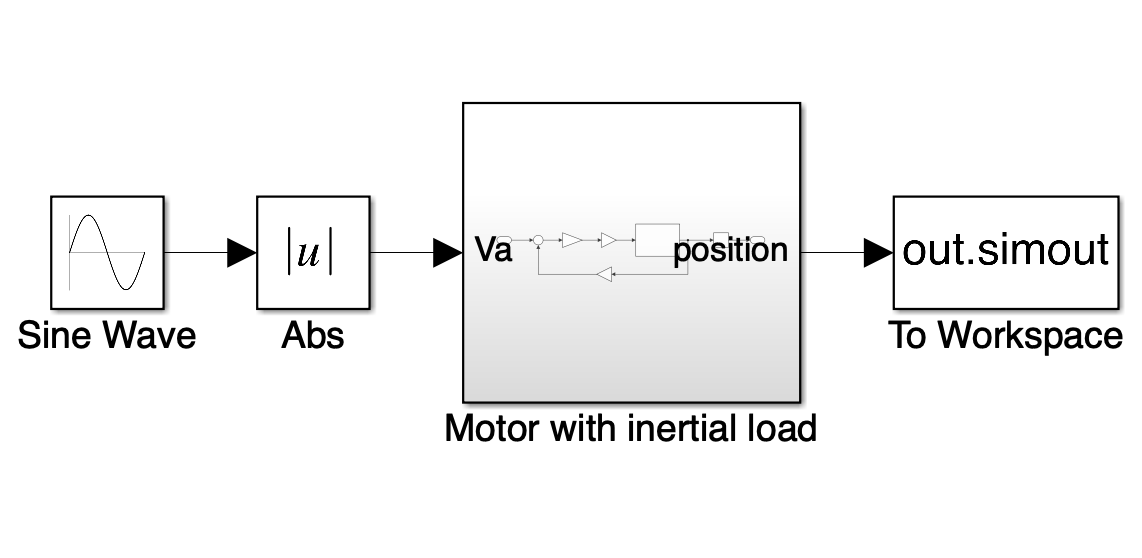
\includegraphics[width=\maxwidth{60.210737581535376em}]{image_0}
\end{flushleft}
\end{par}

\begin{matlabcode}
open_system('motorsim')          % Load the model
out1 = sim('motorsim');
figure                           % Create output figure
plot(out1.simout)
title('motorsim output')
ylabel('Angular Position (rad)')
\end{matlabcode}
\begin{center}
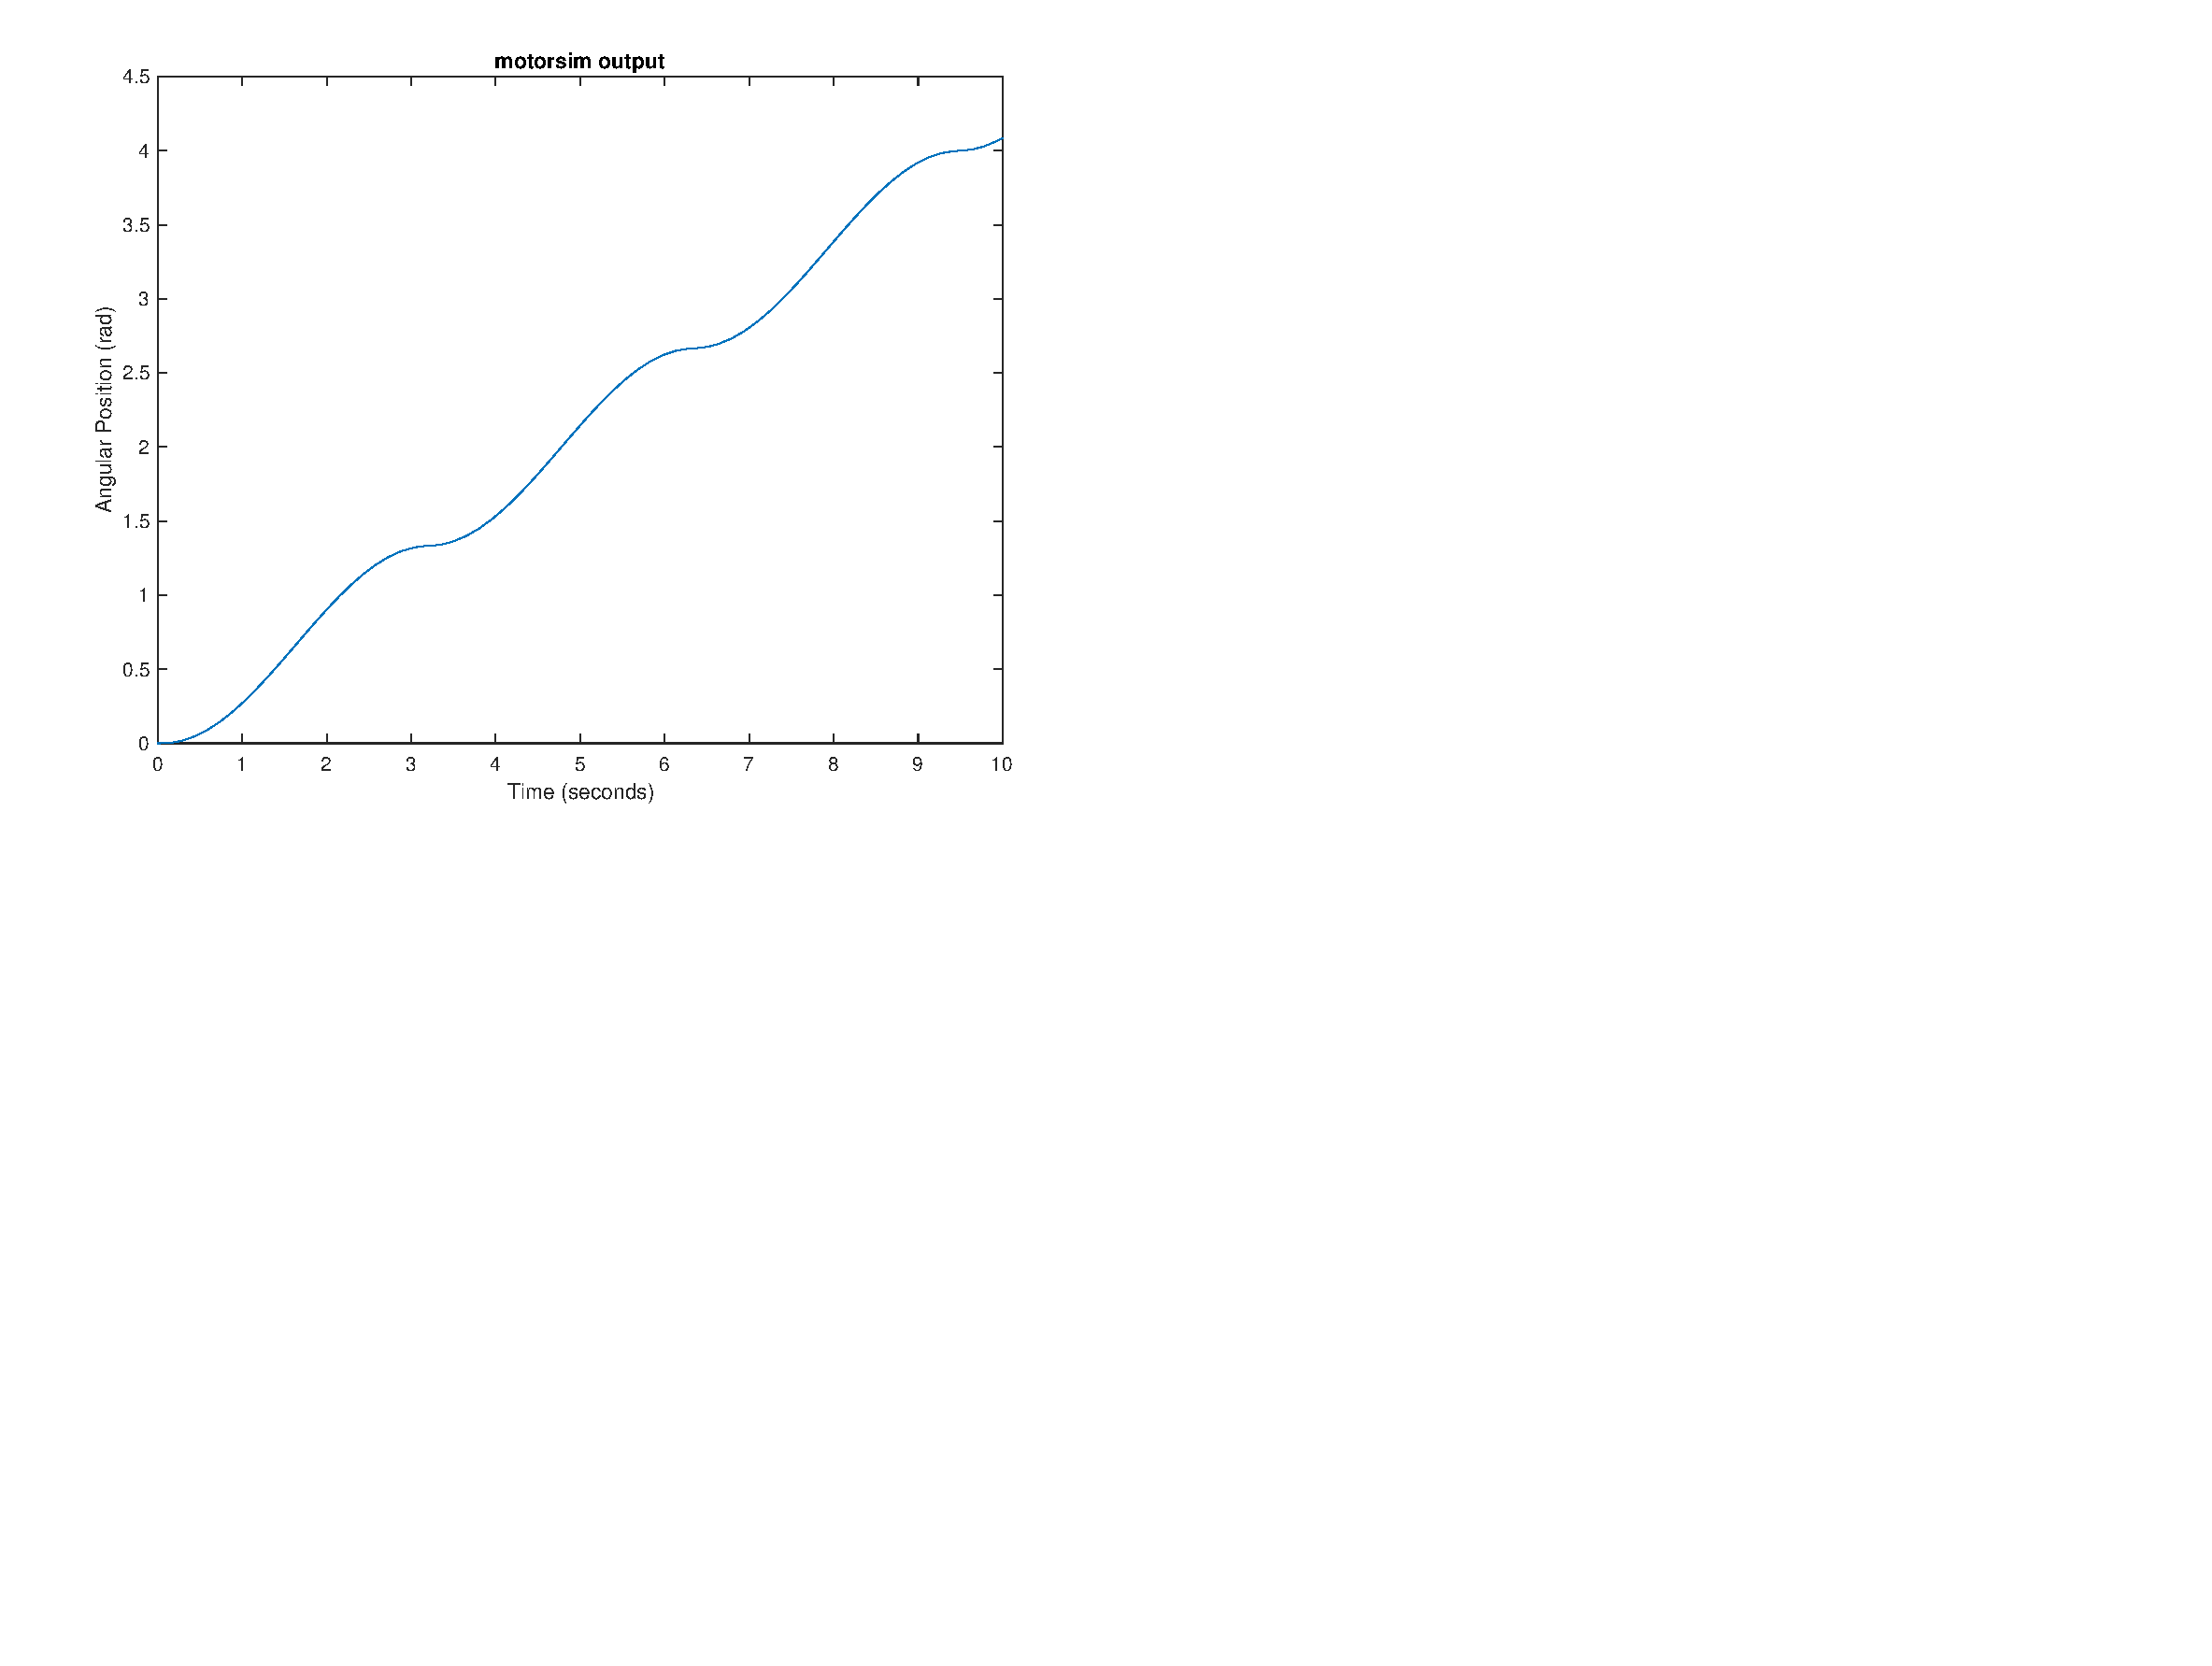
\includegraphics[width=\maxwidth{56.196688409433015em}]{figure_0.eps}
\end{center}

\begin{par}
\begin{flushleft}
The motor rotates in the positive direction, with some oscillations due to the varying input
\end{flushleft}
\end{par}


\matlabheadingthree{Plot of Motor Response with PWM Input}

\begin{par}
\begin{flushleft}
Shows the effect of a continuous PWM input
\end{flushleft}
\end{par}

\begin{par}
\begin{flushleft}
\textit{Requires motorPWM.slx}
\end{flushleft}
\end{par}

\begin{par}
\begin{flushleft}
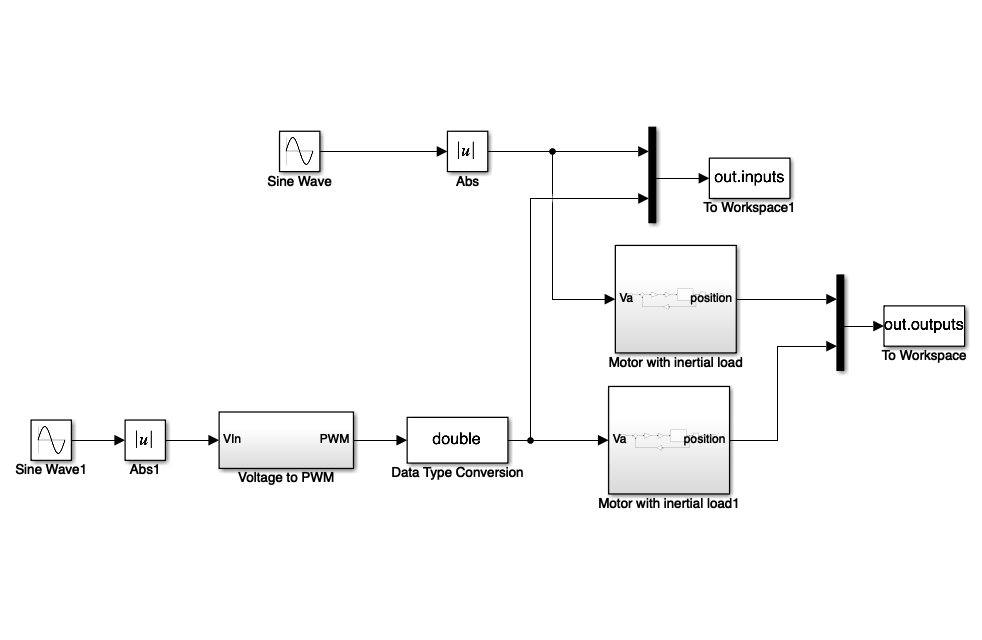
\includegraphics[width=\maxwidth{60.210737581535376em}]{image_1}
\end{flushleft}
\end{par}

\begin{matlabcode}
open_system('motorPWM')         % Load the model 
PWMout = sim('motorPWM');
figure                          % Create input figure
plot(PWMout.inputs)
title('motorPWM Inputs')
ylabel('Amplitude')
\end{matlabcode}
\begin{center}
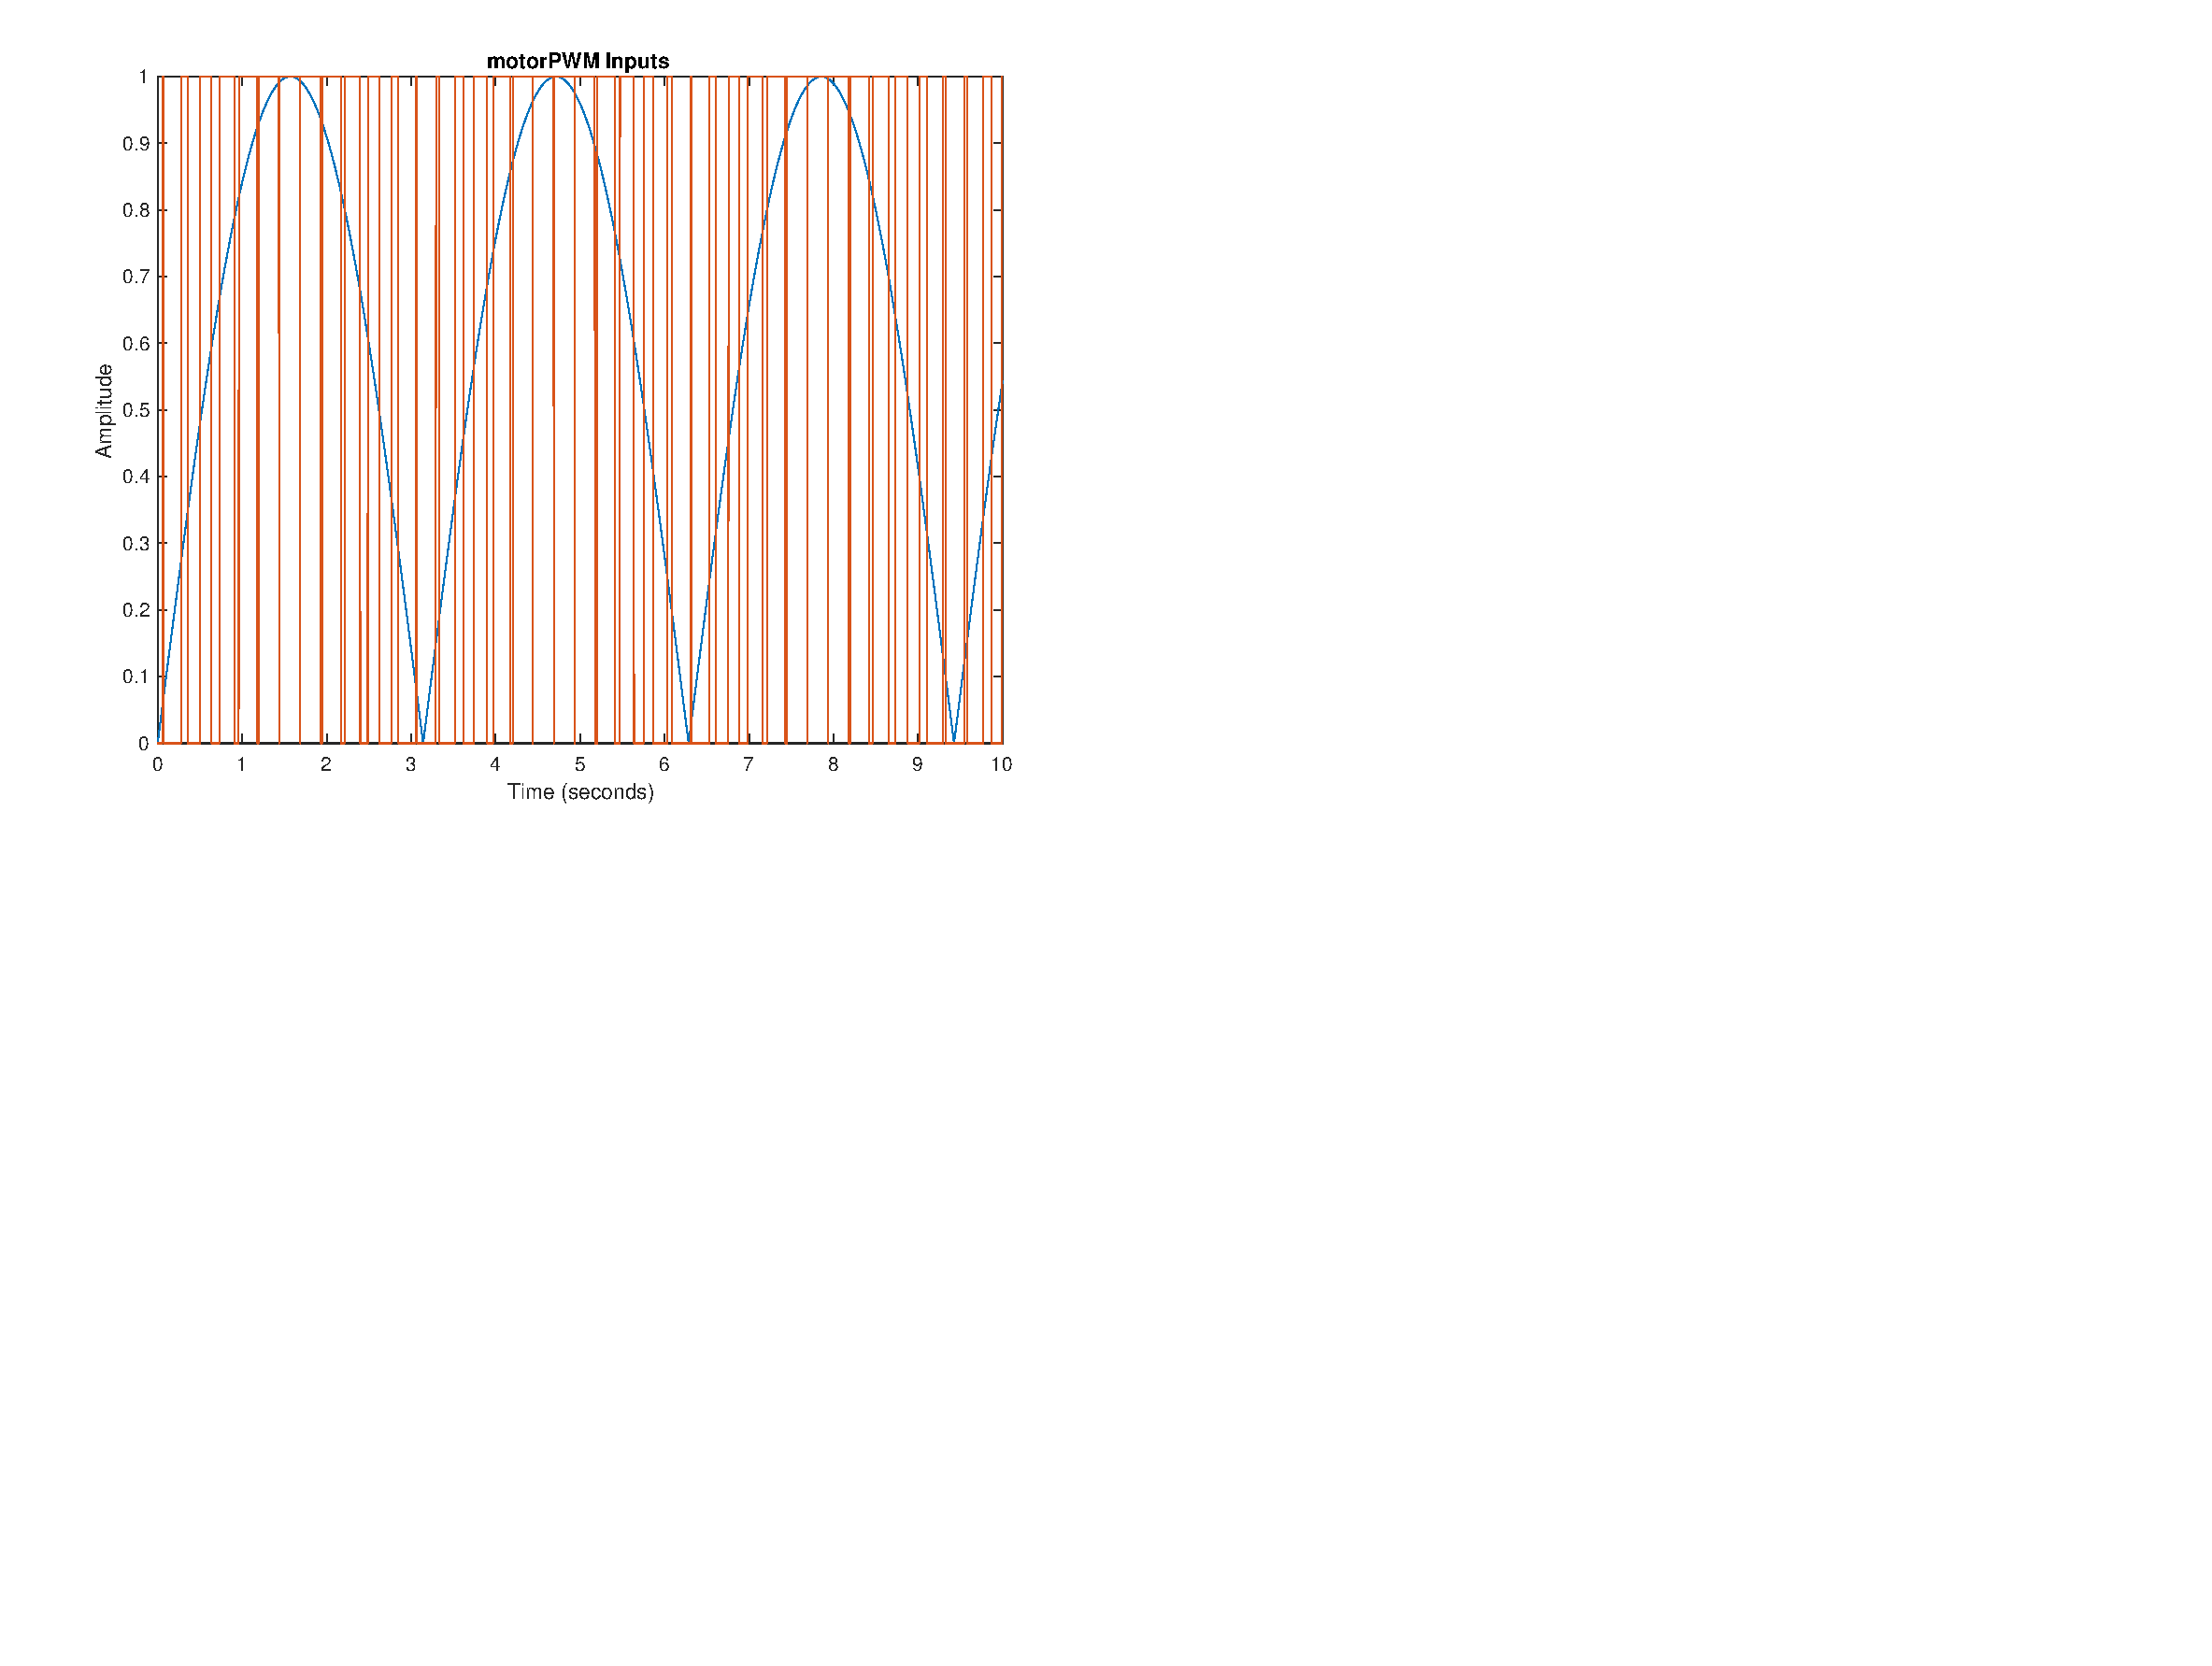
\includegraphics[width=\maxwidth{56.196688409433015em}]{figure_1.eps}
\end{center}
\begin{matlabcode}
figure                          % Create output figure
plot(PWMout.outputs)
title('motorPWM Outputs')
ylabel('Amplitude')
\end{matlabcode}
\begin{center}
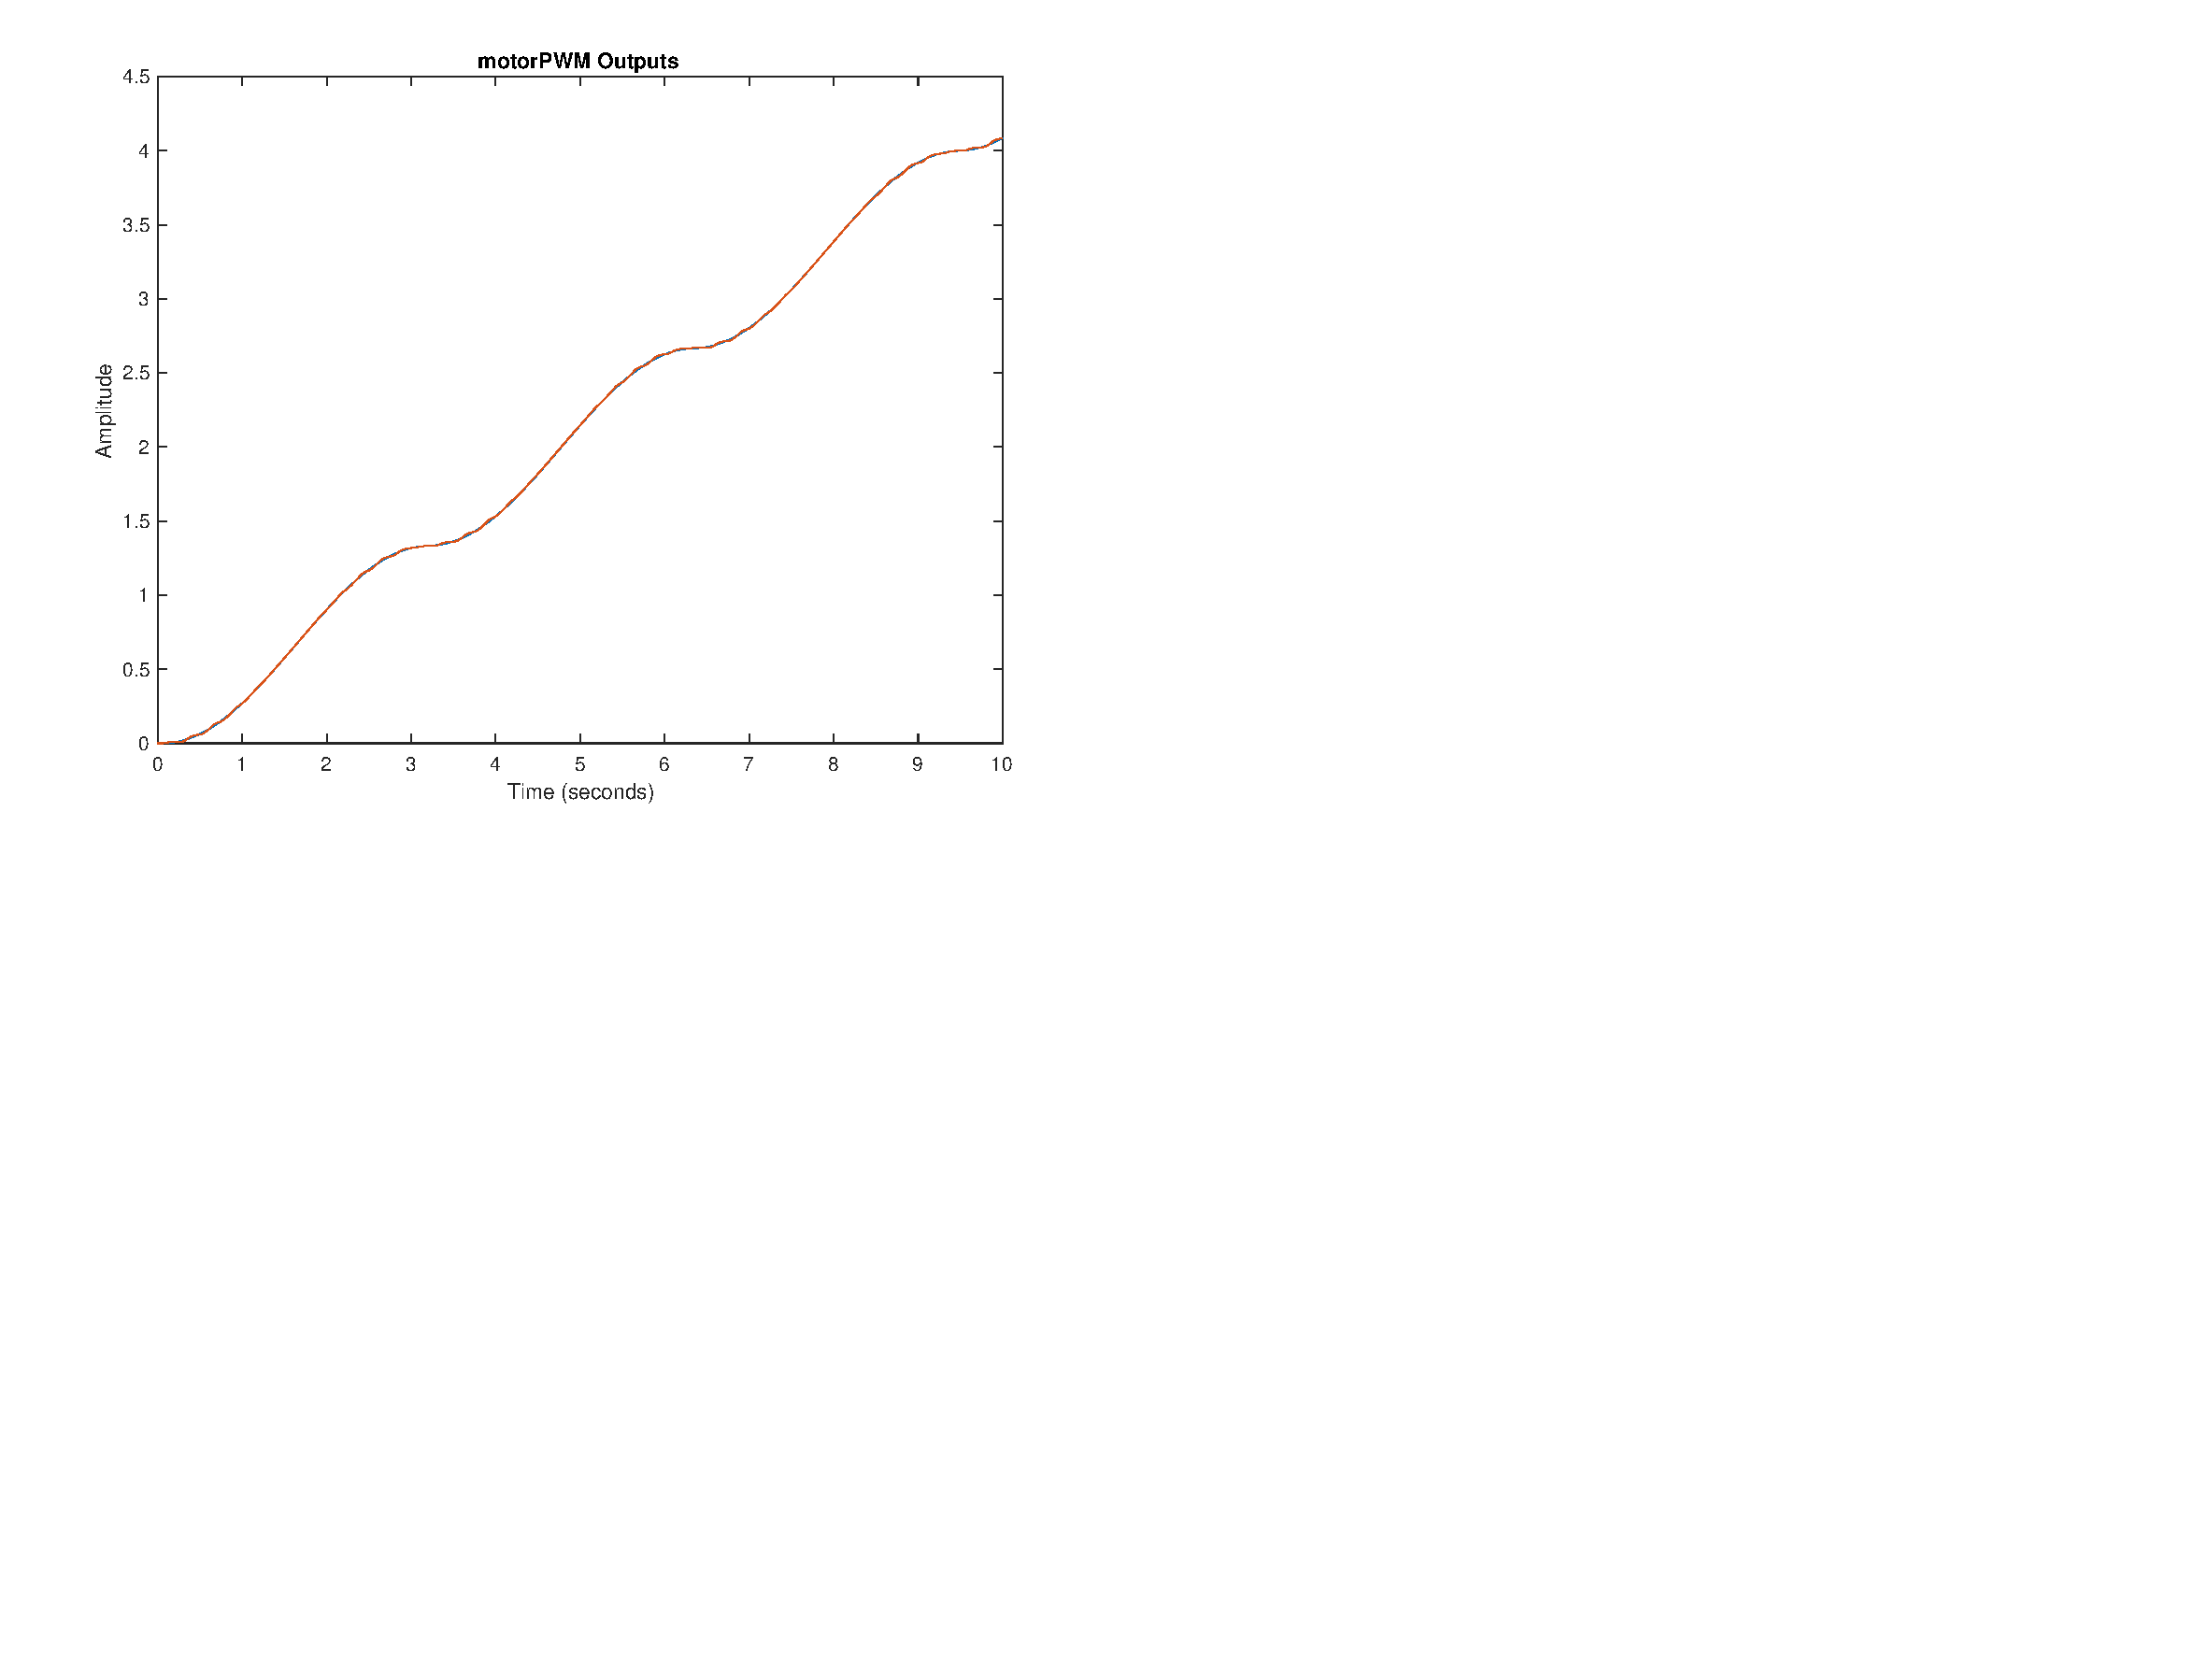
\includegraphics[width=\maxwidth{56.196688409433015em}]{figure_2.eps}
\end{center}


\matlabheadingthree{Plot of Motor Response with Quantized Input}

\begin{par}
\begin{flushleft}
Shows the effect of a quantized input
\end{flushleft}
\end{par}

\begin{par}
\begin{flushleft}
\textit{Requires motorQuantized.slx}
\end{flushleft}
\end{par}

\begin{par}
\begin{flushleft}
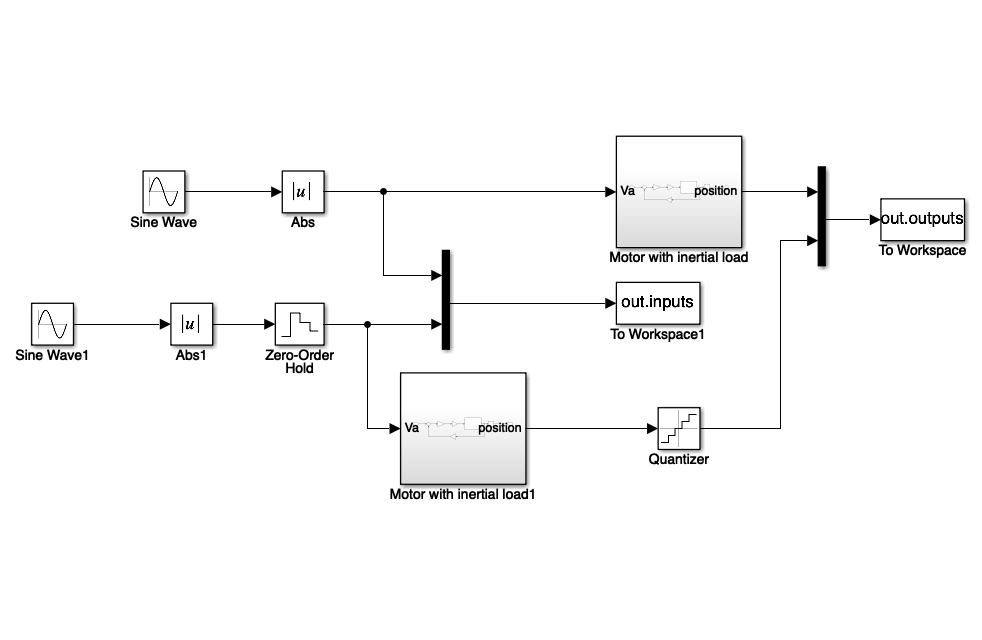
\includegraphics[width=\maxwidth{60.210737581535376em}]{image_2}
\end{flushleft}
\end{par}

\begin{matlabcode}
open_system('motorQuantized')   % Load the model
Qout = sim('motorQuantized');
figure                          % Create input figure
plot(Qout.inputs)
title('motorQuantized Inputs')
ylabel('Amplitude')
\end{matlabcode}
\begin{center}
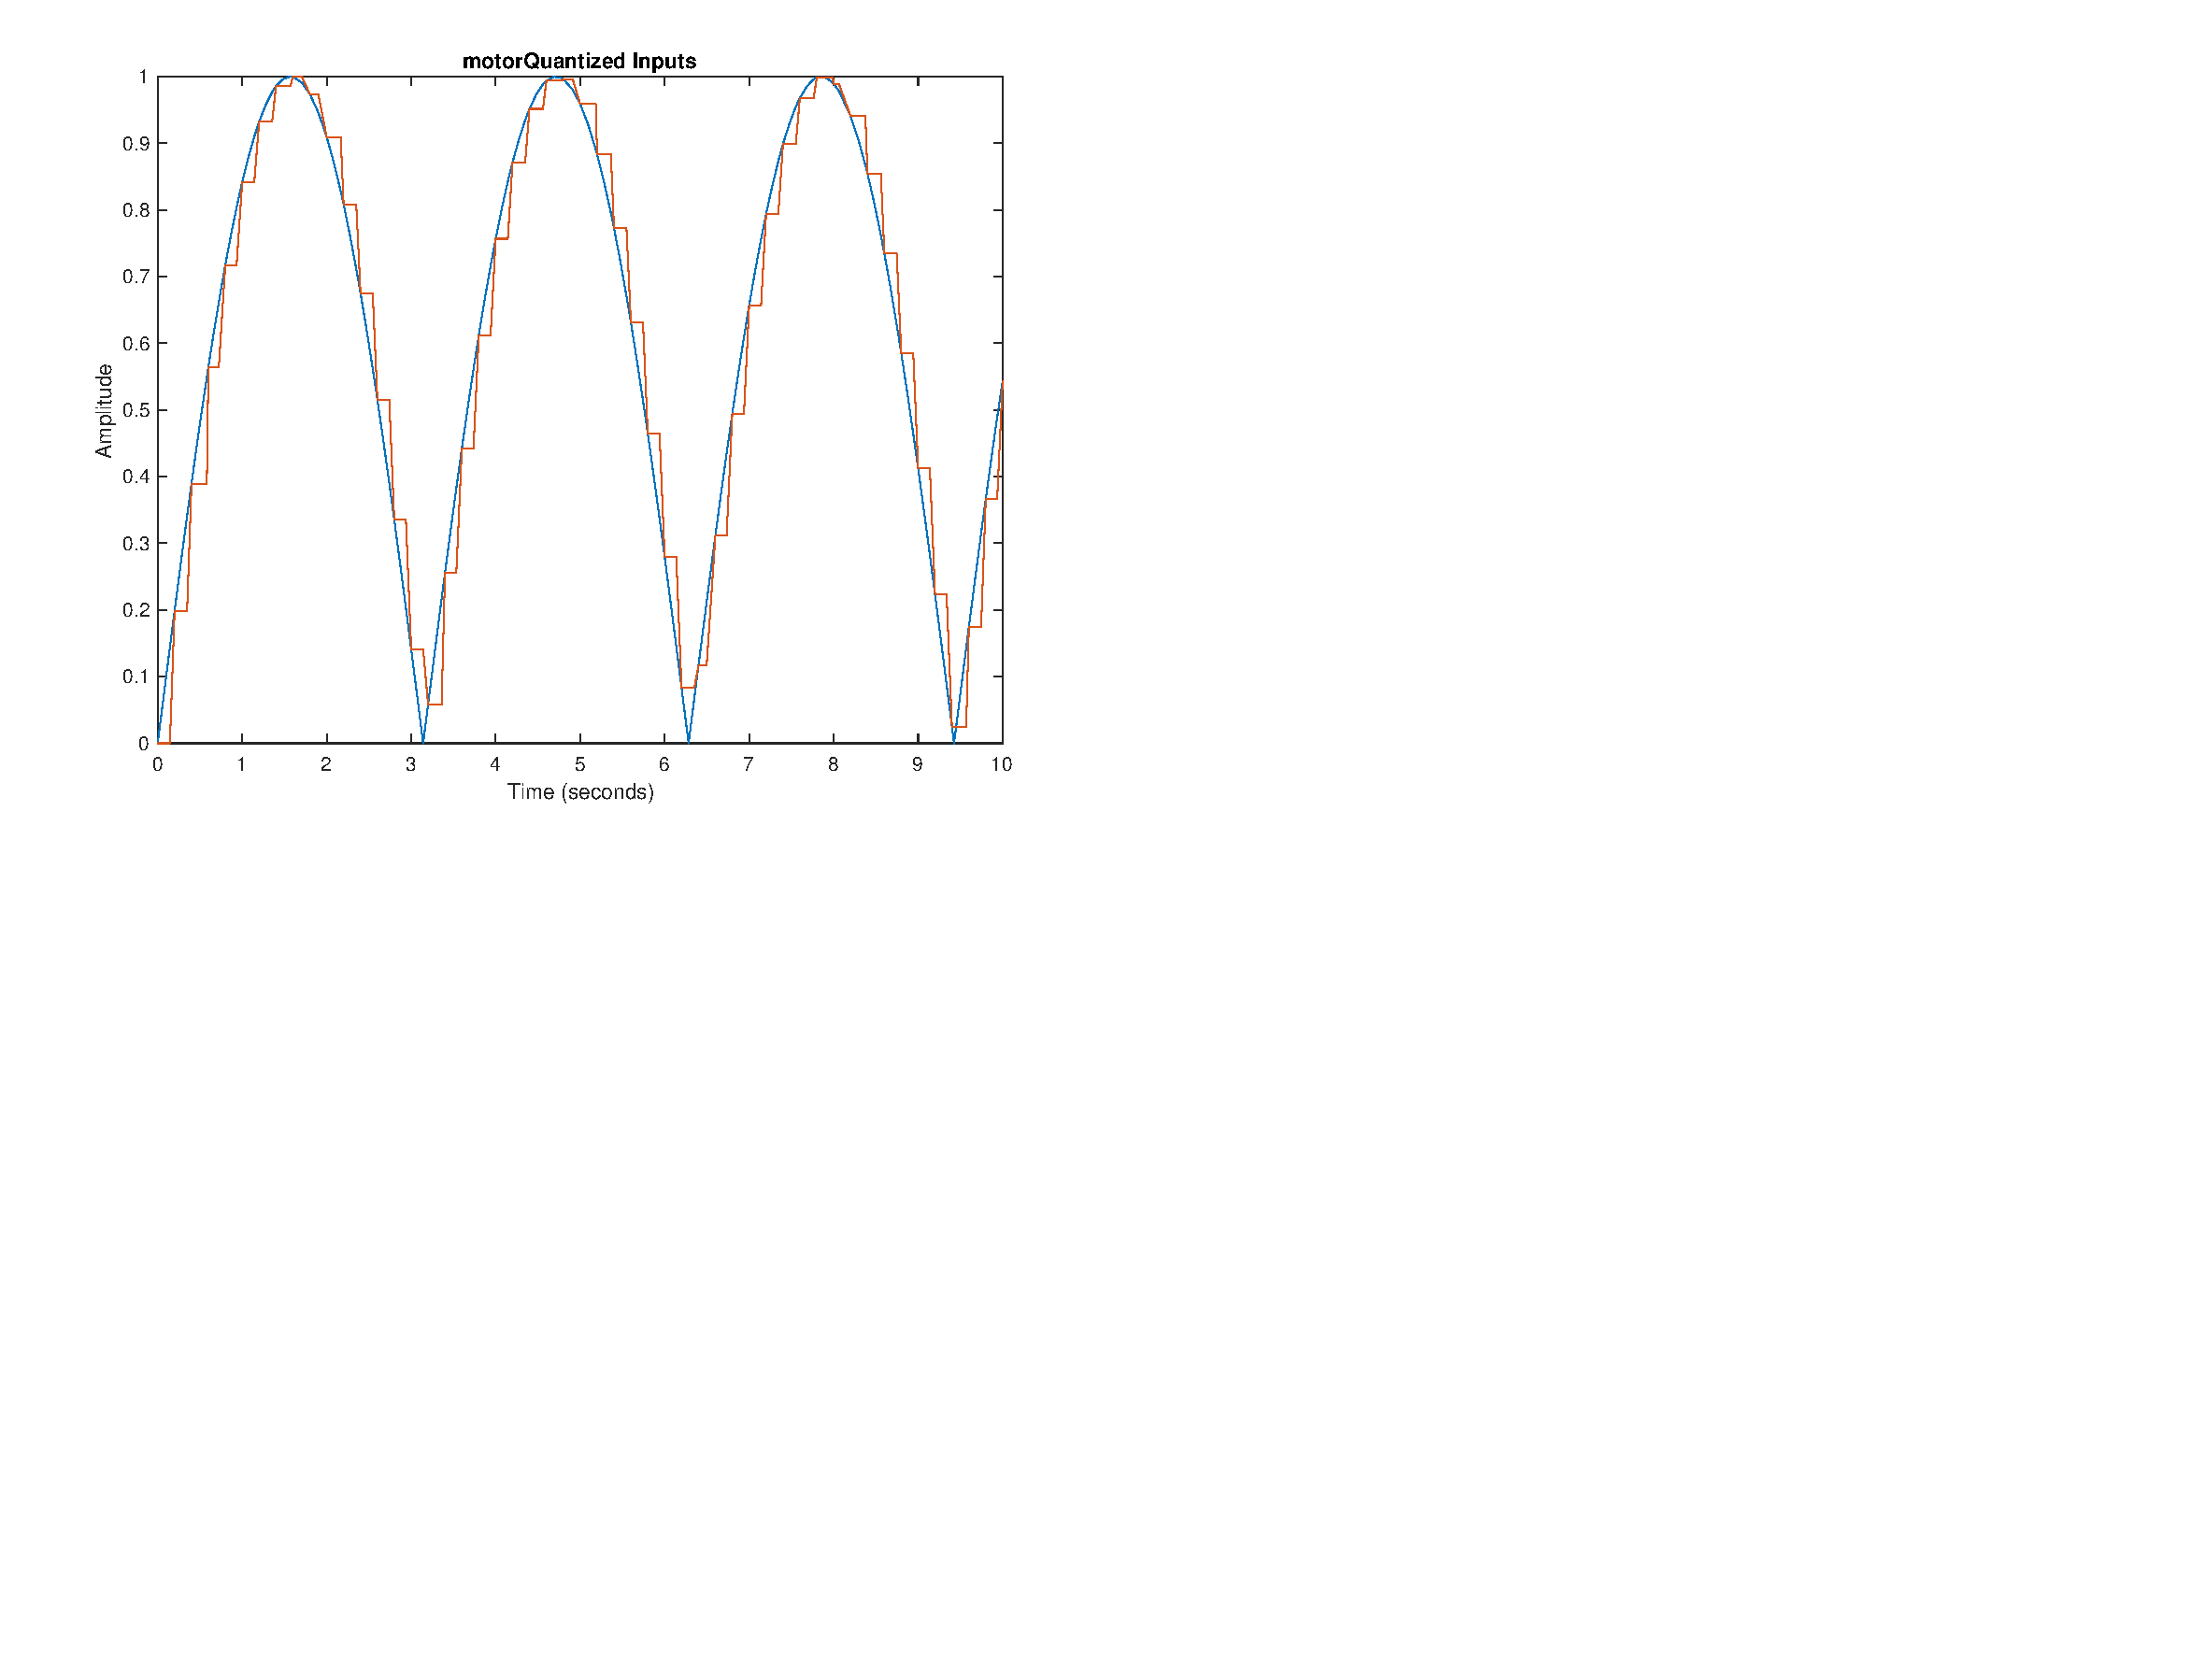
\includegraphics[width=\maxwidth{56.196688409433015em}]{figure_3.eps}
\end{center}
\begin{matlabcode}
figure                          % Create output figure
plot(Qout.outputs)
title('motorQuantized Outputs')
ylabel('Amplitude')
\end{matlabcode}
\begin{center}
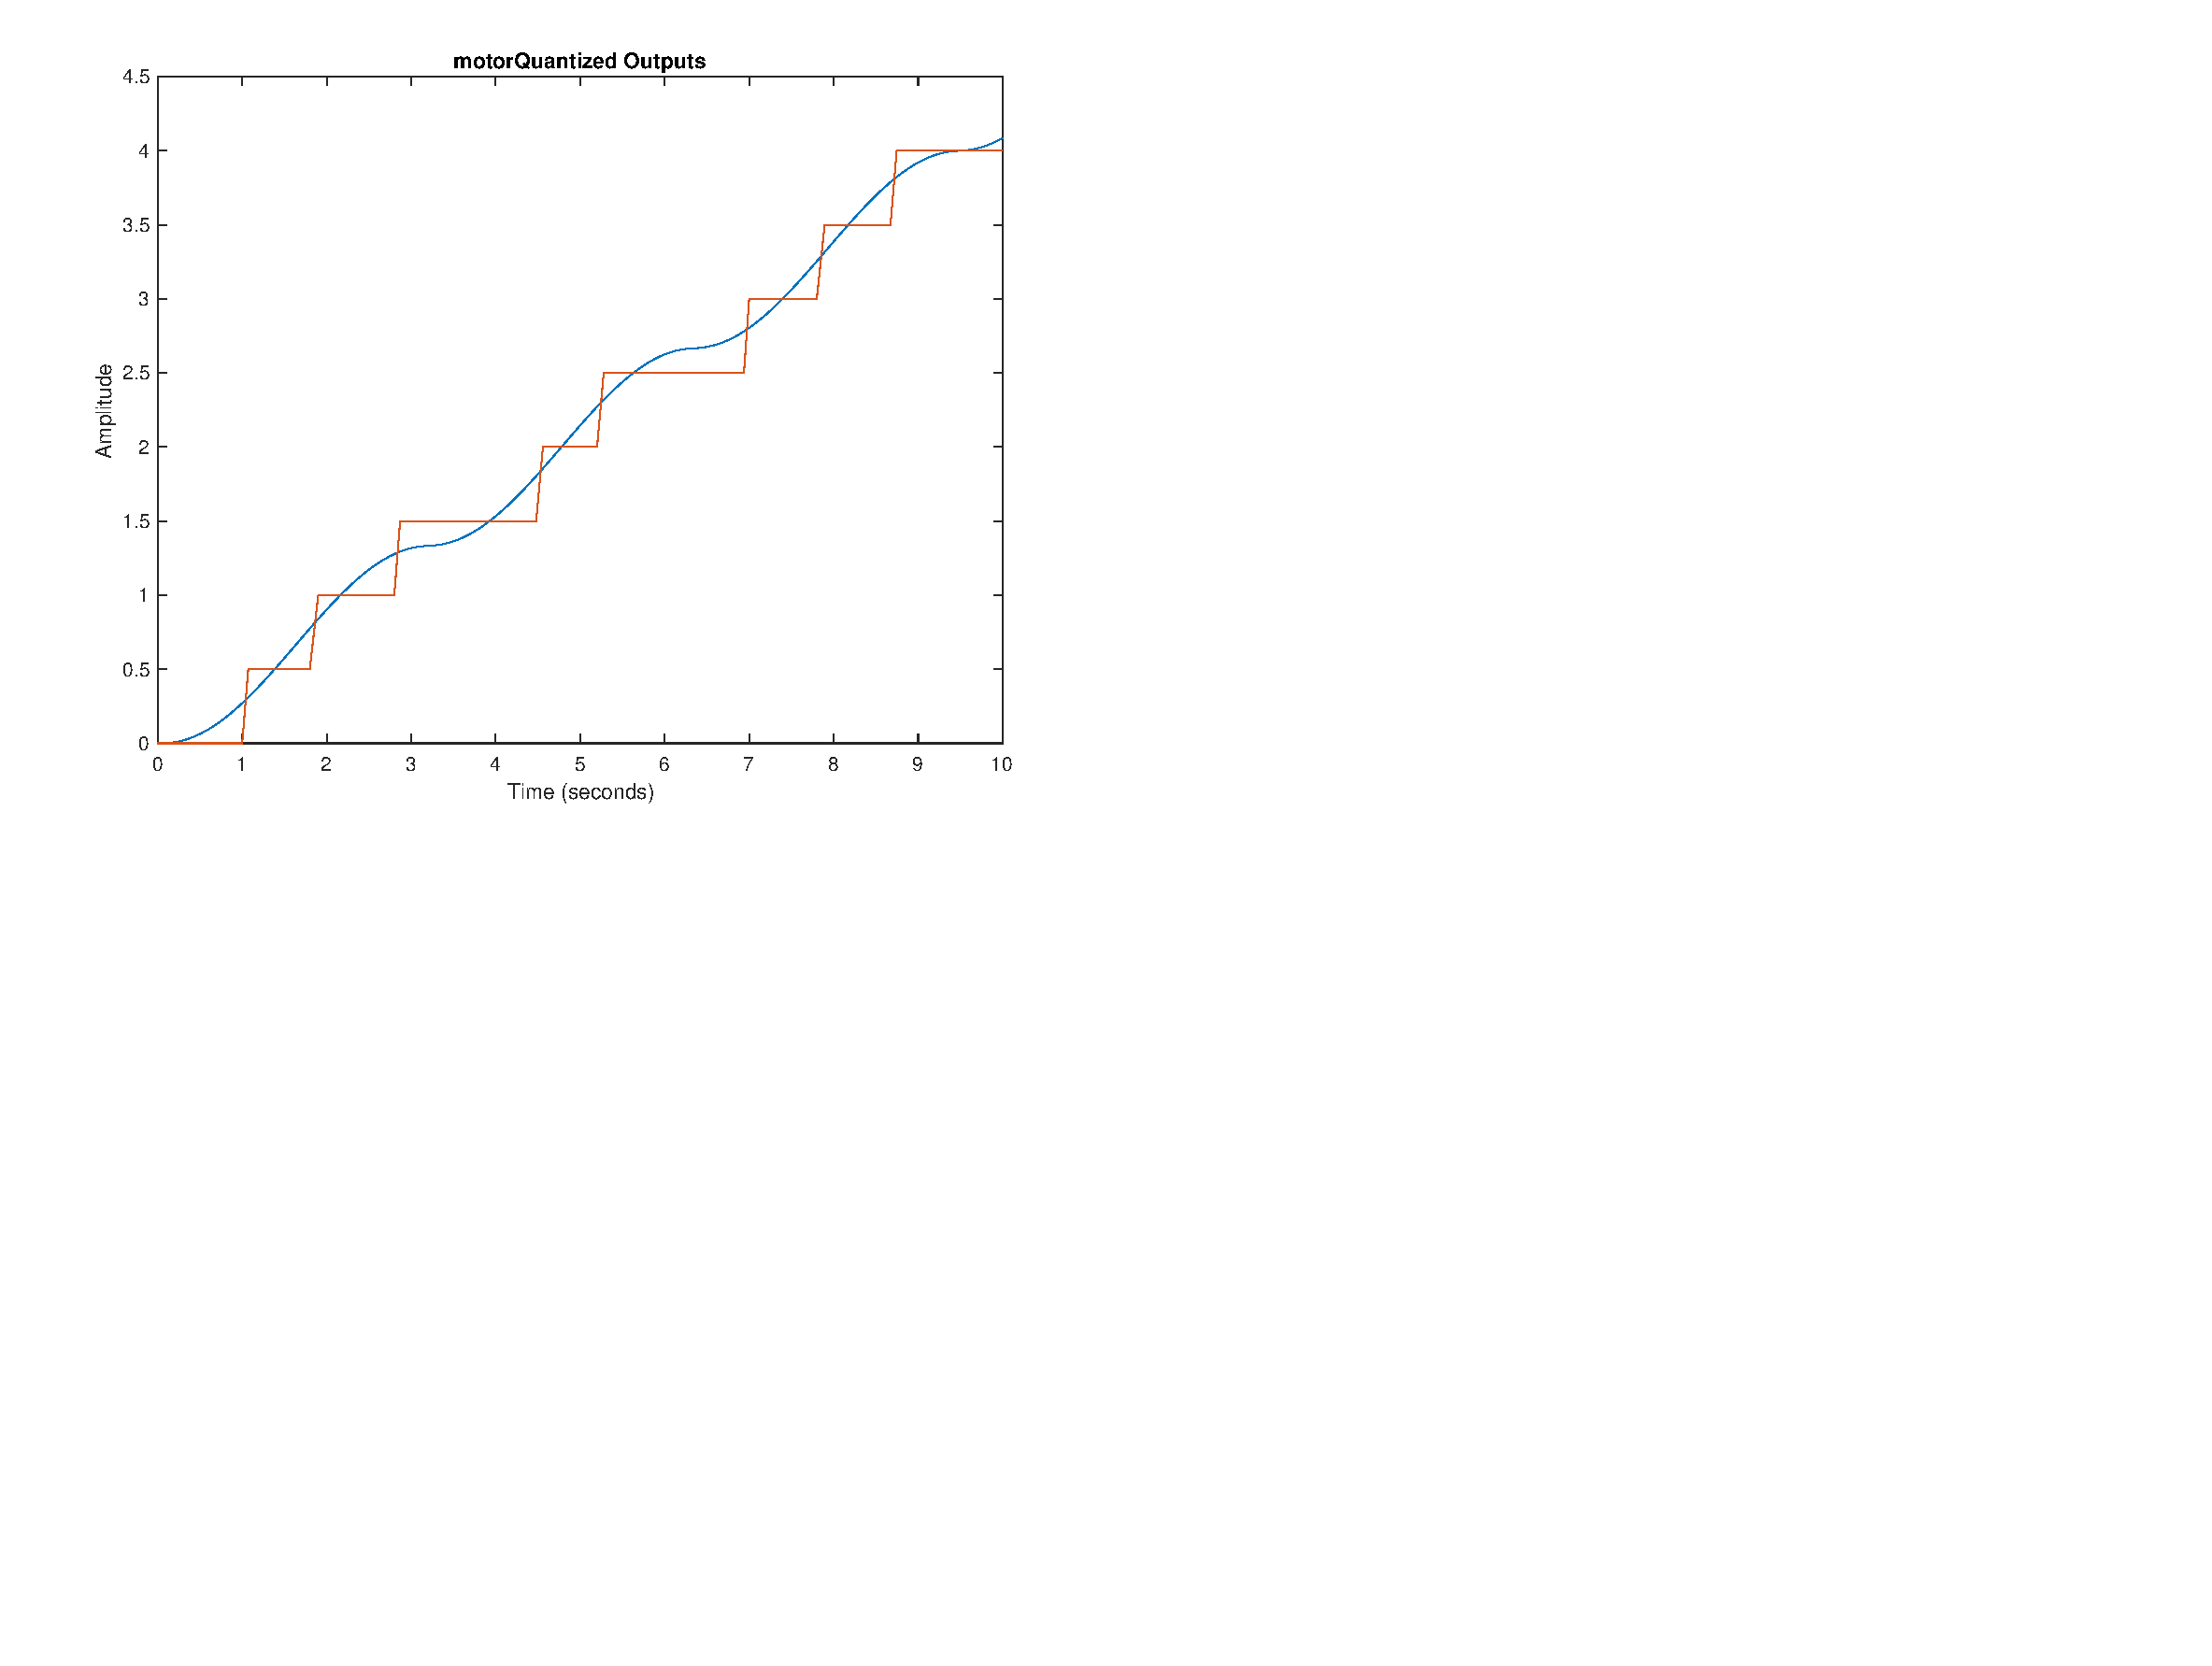
\includegraphics[width=\maxwidth{56.196688409433015em}]{figure_4.eps}
\end{center}

\begin{par}
\begin{flushleft}
A quantized input is an approximation of the continuous input, and although it requires fewer points, it isn't very useful.
\end{flushleft}
\end{par}


\matlabheadingthree{Finding the Transfer Function of the Motor}

\begin{par}
\begin{flushleft}
Using slLinearizer and getIOTransfer, MATLAB will find the closed loop transfer function of the motor for me!
\end{flushleft}
\end{par}

\begin{par}
\begin{flushleft}
\textit{Requires motor.slx}
\end{flushleft}
\end{par}

\begin{par}
\begin{flushleft}
motor is the "Motor" subsystem
\end{flushleft}
\end{par}

\begin{par}
\begin{flushleft}
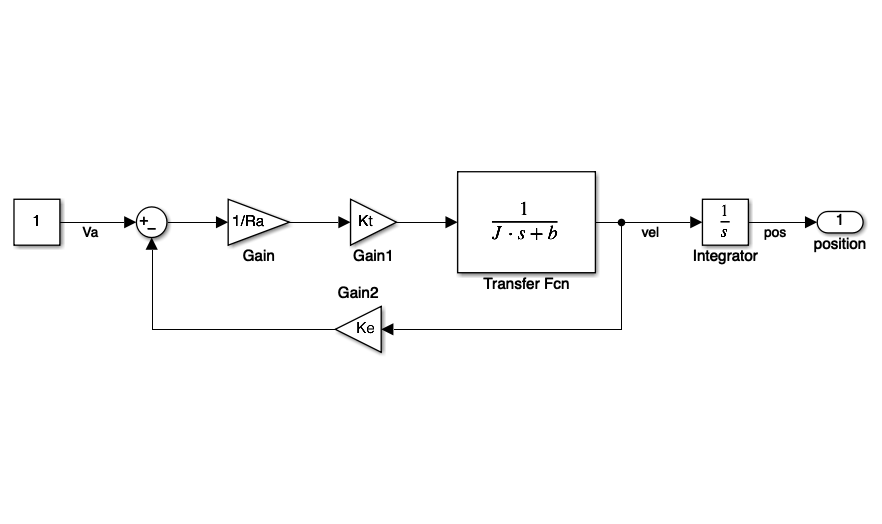
\includegraphics[width=\maxwidth{60.210737581535376em}]{image_3}
\end{flushleft}
\end{par}

\begin{matlabcode}
open_system('motor');                       % Load the model
sllin = slLinearizer('motor');              % Create new a slLinearizer model
addPoint(sllin,{'Va','pos','vel'});         % Label the reference input and block output
posTF = getIOTransfer(sllin,'Va','pos');    % Use getIOTransfer to find TF of Pos/Va
velTF = getIOTransfer(sllin,'Va','vel');    % Use getIOTransfer to find TF of Vel/Va
\end{matlabcode}

\begin{par}
\begin{flushleft}
Turn the generated position transfer function into a coefficient array for use in Simulink.
\end{flushleft}
\end{par}

\begin{matlabcode}
posTF = tf(posTF)                           % Convert to a TF object
\end{matlabcode}
\begin{matlaboutput}
posTF =
 
  From input "Va" to output "pos":
      10
  ----------
  s^2 + 15 s
 
Continuous-time transfer function.
\end{matlaboutput}
\begin{matlabcode}
posNum = posTF.Numerator;                   % Find the numerator coefficients
posNum = posNum{1};                         % Convert the numerator to a the right form
posDen = posTF.Denominator;                 % Find the denominator coefficients
posDen = posDen{1};                         % Convert the denominator to a the right form
\end{matlabcode}

\begin{par}
\begin{flushleft}
Turn the generated velocity transfer function into a coefficient array for use in Simulink.
\end{flushleft}
\end{par}

\begin{matlabcode}
velTF = tf(velTF)                           % Convert to a TF object
\end{matlabcode}
\begin{matlaboutput}
velTF =
 
  From input "Va" to output "vel":
    10
  ------
  s + 15
 
Continuous-time transfer function.
\end{matlaboutput}
\begin{matlabcode}
velNum = velTF.Numerator;                   % Find the numerator coefficients
velNum = velNum{1};                         % Convert the numerator to a the right form
velDen = velTF.Denominator;                 % Find the denominator coefficients
velDen = velDen{1};                         % Convert the denominator to a the right form
\end{matlabcode}


\matlabheadingthree{Plots of Motor Vs. Transfer Function - Position and Velocity}

\begin{par}
\begin{flushleft}
\textit{Requires motorWithTF.slx}
\end{flushleft}
\end{par}

\begin{par}
\begin{flushleft}
Compares the generated transfer function with the baseline motor response.
\end{flushleft}
\end{par}

\begin{par}
\begin{flushleft}
(Red is the transfer function response, blue is the motor response)
\end{flushleft}
\end{par}

\begin{par}
\begin{flushleft}
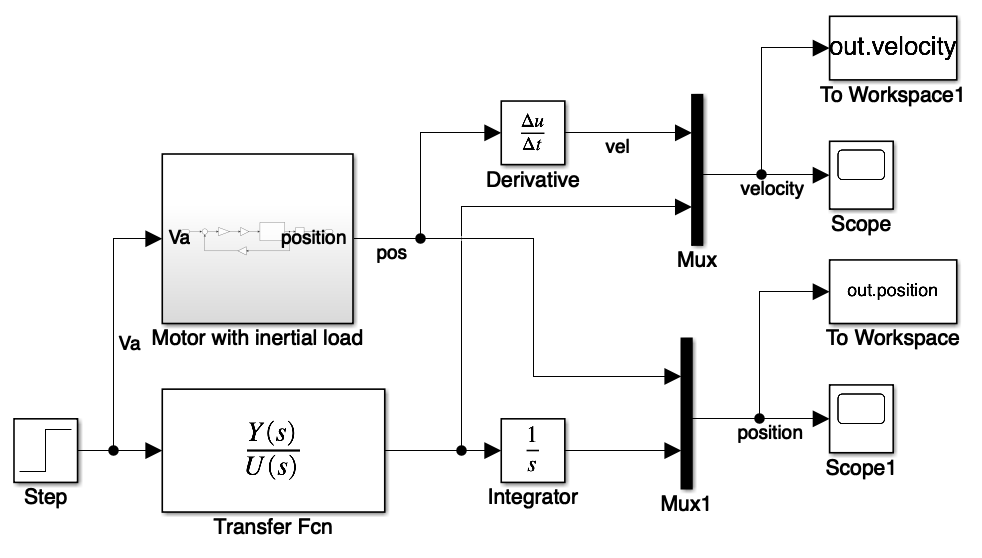
\includegraphics[width=\maxwidth{60.210737581535376em}]{image_4}
\end{flushleft}
\end{par}


\vspace{1em}
\begin{matlabcode}
open_system('motorWithTF')                  % Load the model
motorAndTFout = sim('motorWithTF');
figure                                      % Create the position figure 
plot(motorAndTFout.position)
title('motorWithTF Position')
\end{matlabcode}
\begin{center}
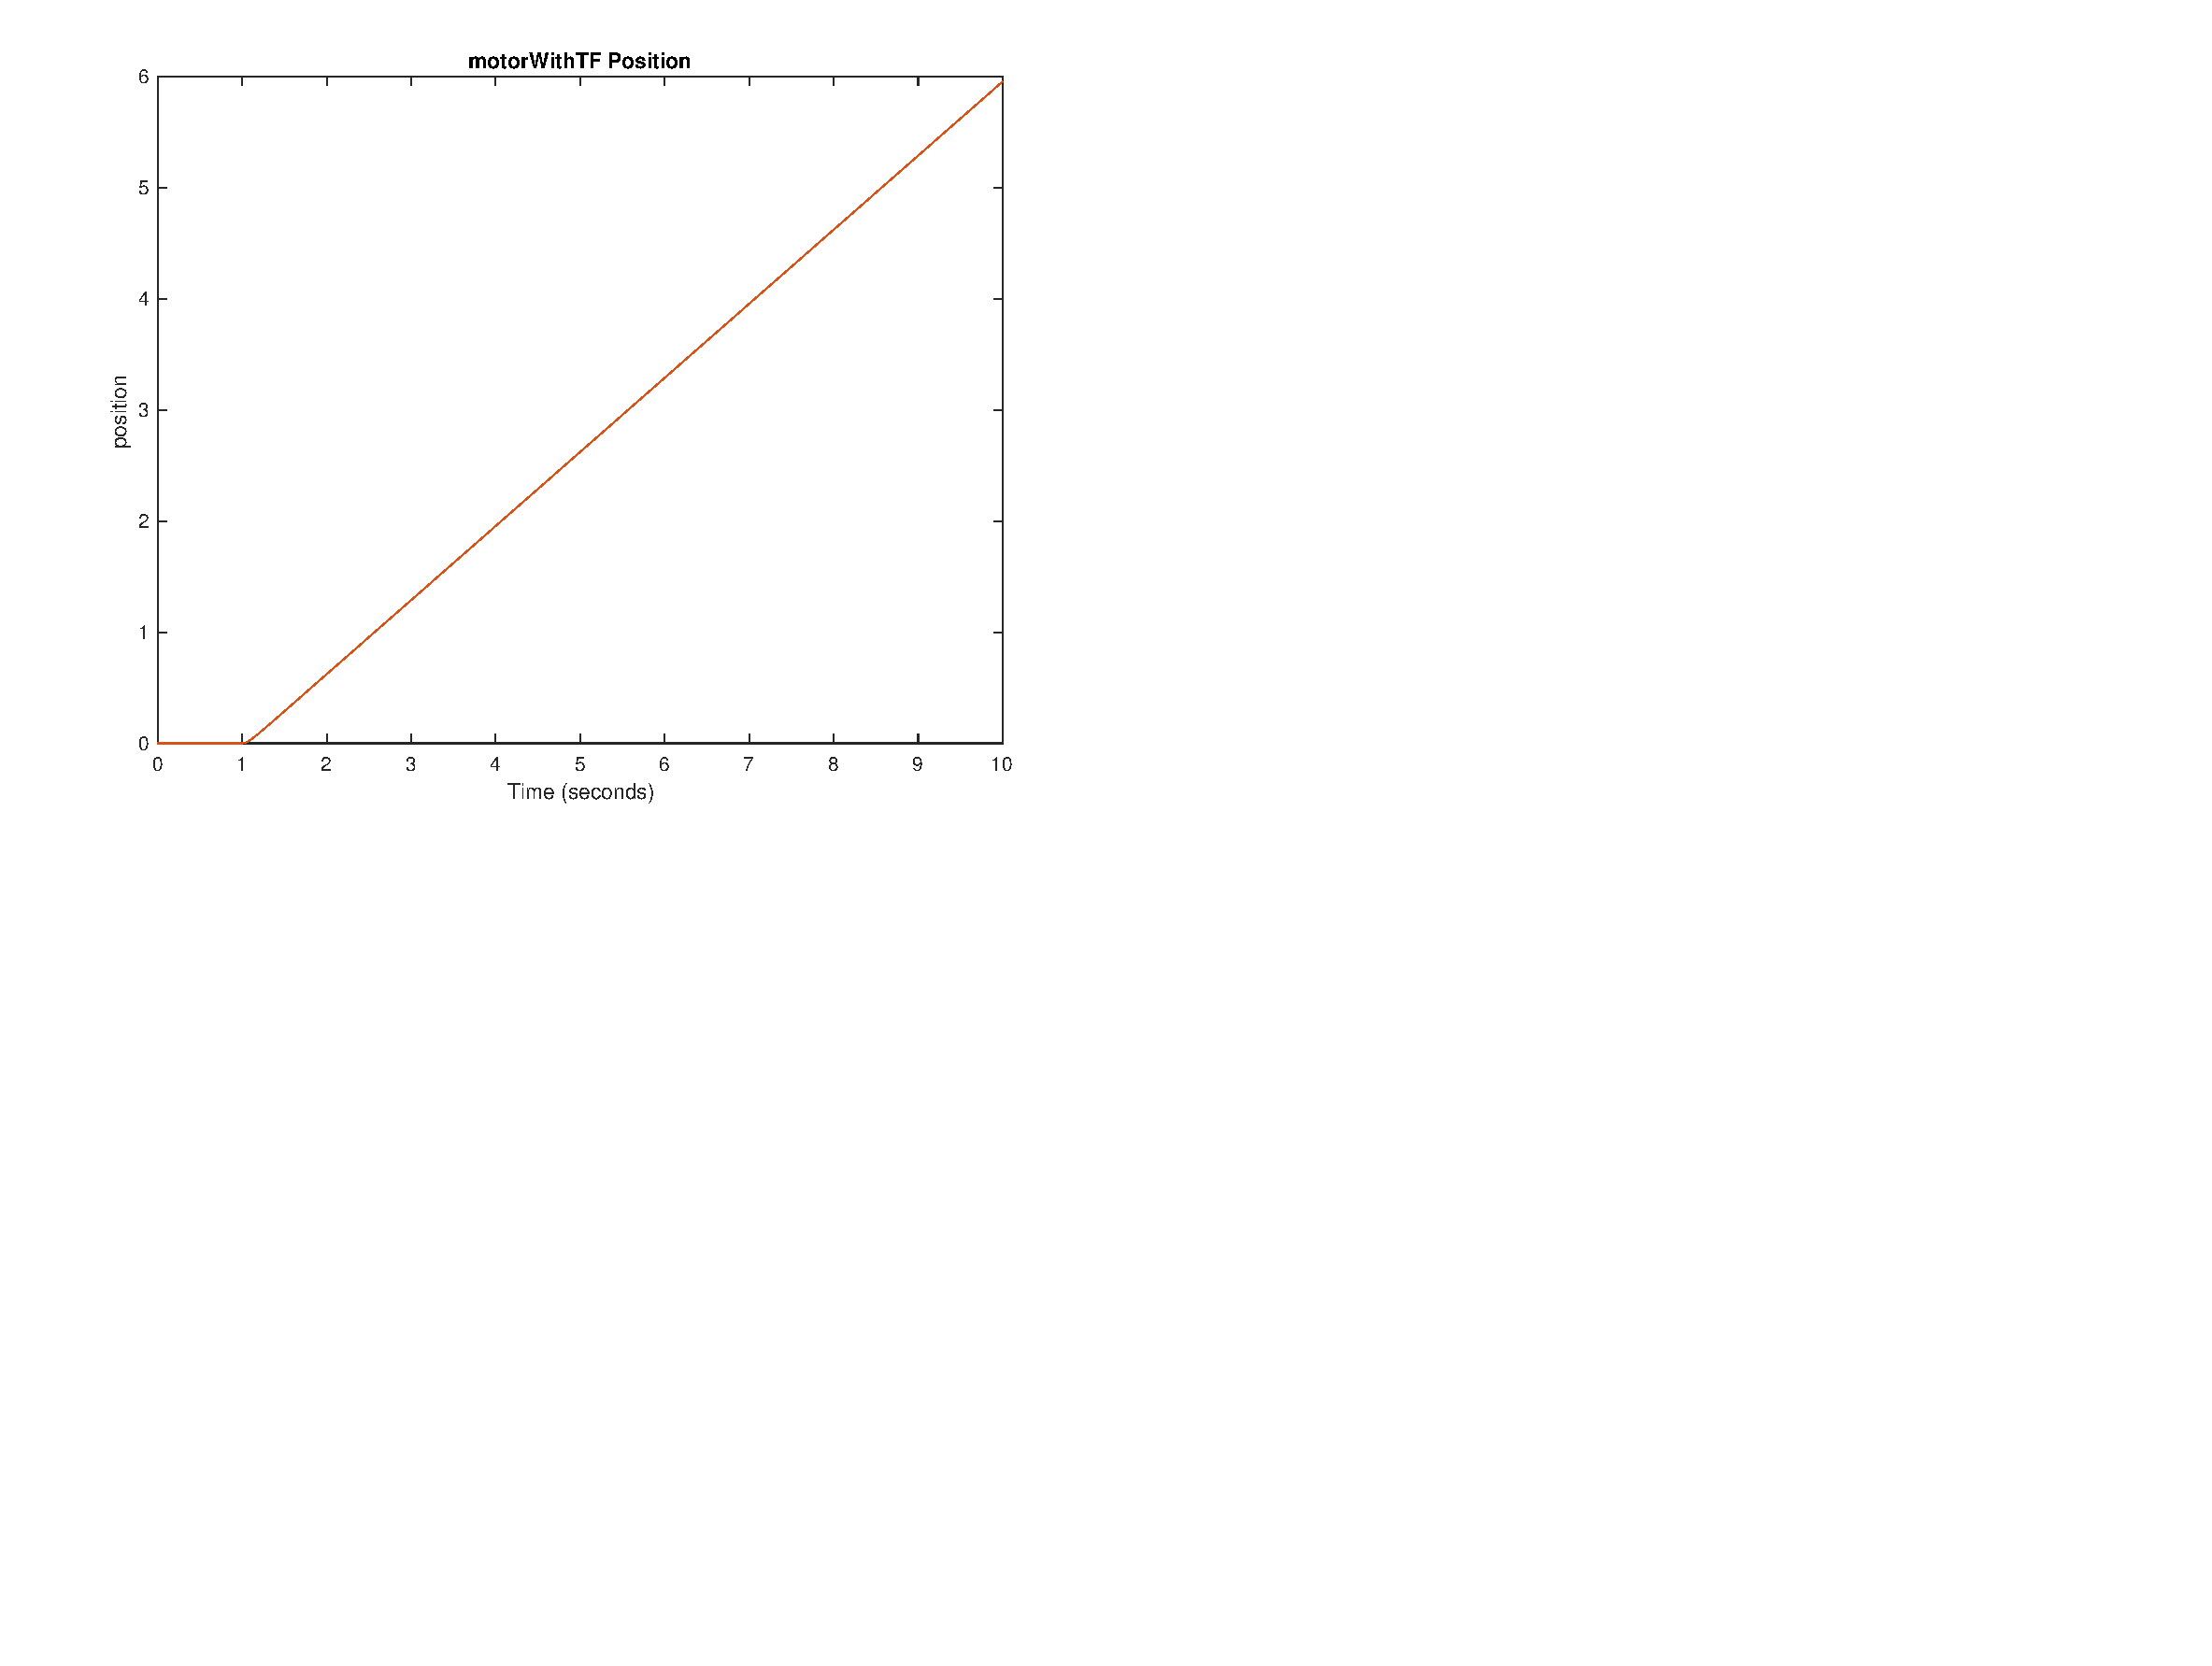
\includegraphics[width=\maxwidth{56.196688409433015em}]{figure_5.eps}
\end{center}
\begin{matlabcode}
figure                                      % Create the velocity figure
plot(motorAndTFout.velocity)
title('motorWithTF Velocity')
\end{matlabcode}
\begin{center}
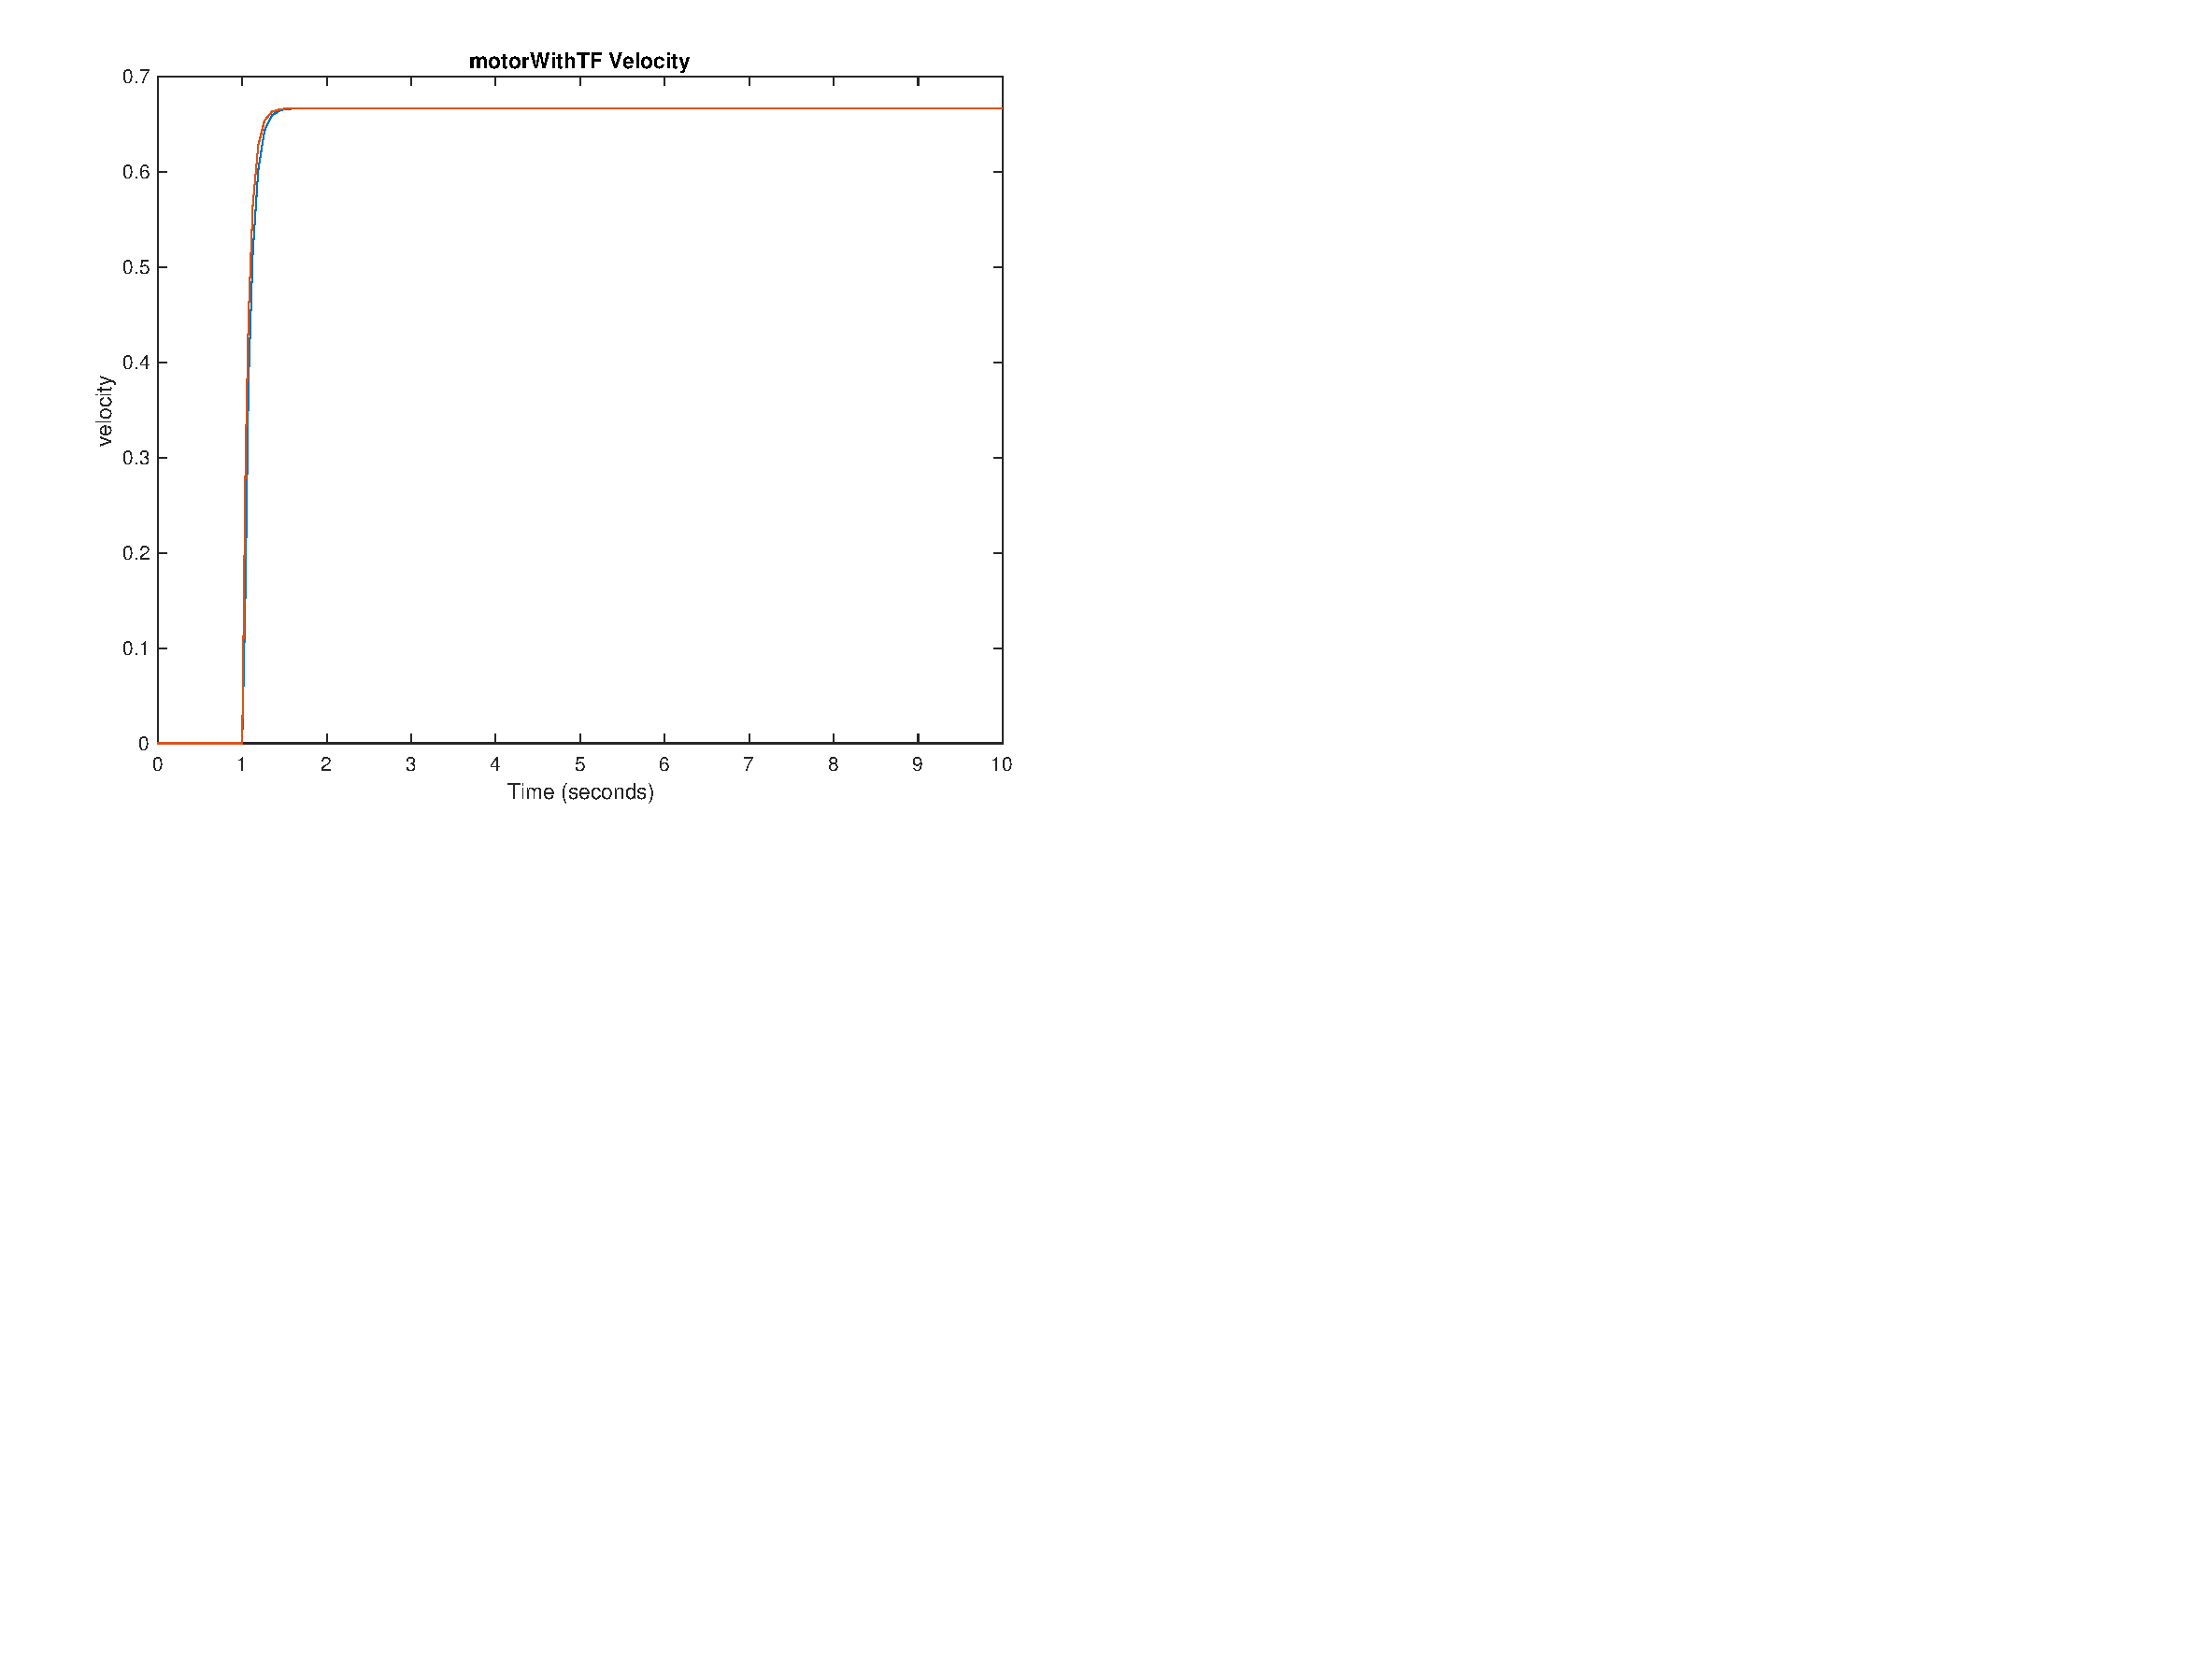
\includegraphics[width=\maxwidth{56.196688409433015em}]{figure_6.eps}
\end{center}


\matlabheadingthree{Creating and Tuning a PI controller for Motor}

\begin{par}
\begin{flushleft}
Why open pidTuner in a new window when I can do it inline
\end{flushleft}
\end{par}

\begin{matlabcode}
% Convert Response Time to Bandwidth
% Bandwidth is equivalent to 2 divided by the Response Time
wc = 2/0.411919;

% Convert Transient Behavior to Phase Margin
% Phase Margin is equivalent to the Transient Behavior multiplied by 100
PM = 100*0.659116;

% Define options for pidtune command
opts = pidtuneOptions('PhaseMargin',PM);

% PID tuning algorithm for linear plant model
[CI,pidInfo] = pidtune(posTF,'PI',wc,opts);

% Clear Temporary Variables
clear wc PM opts

% Get desired loop response
Response = getPIDLoopResponse(CI,posTF,'closed-loop');

% Plot the result
stepplot(Response)
title('Step Plot: Reference tracking')
grid on
\end{matlabcode}
\begin{center}
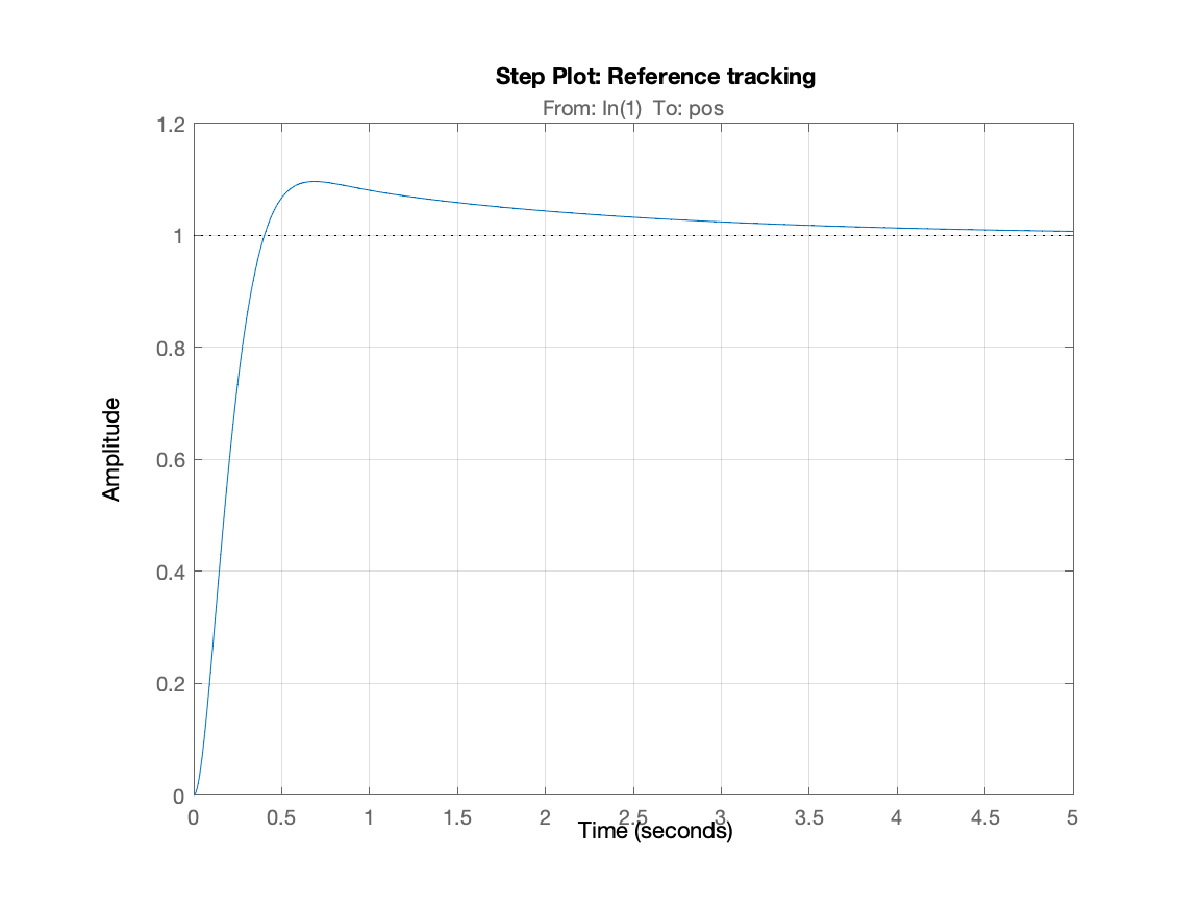
\includegraphics[width=\maxwidth{56.196688409433015em}]{figure_7.eps}
\end{center}
\begin{matlabcode}

% Display system response characteristics
disp(stepinfo(Response))
\end{matlabcode}
\begin{matlaboutput}
         RiseTime: 0.2675
    TransientTime: 3.3361
     SettlingTime: 3.3361
      SettlingMin: 0.9096
      SettlingMax: 1.0967
        Overshoot: 9.6683
       Undershoot: 0
             Peak: 1.0967
         PeakTime: 0.6839
\end{matlaboutput}
\begin{matlabcode}

% Clear Temporary Variables
clear Response
Kp = CI.Kp          % Displays the proportial coeficcient
\end{matlabcode}
\begin{matlaboutput}
Kp = 7.6109
\end{matlaboutput}
\begin{matlabcode}
Ki = CI.Ki          % Displays the integral coeficcient
\end{matlabcode}
\begin{matlaboutput}
Ki = 3.9833
\end{matlaboutput}


\matlabheadingthree{Plot of PI Controled Motor Vs. Transfer Function - Position}

\begin{par}
\begin{flushleft}
The two lines occupy the exact same space on the plot which indicates the generated transfer function is correct.
\end{flushleft}
\end{par}

\begin{par}
\begin{flushleft}
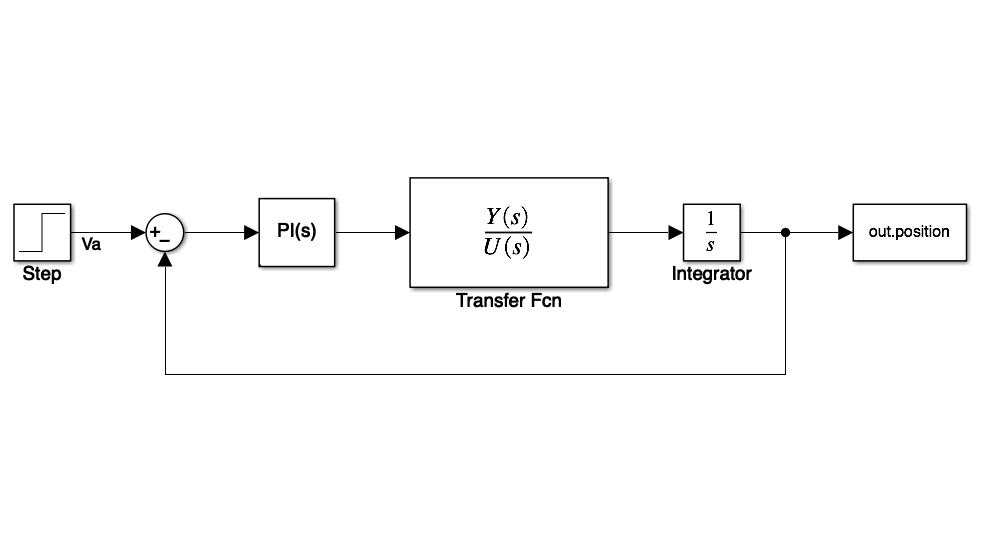
\includegraphics[width=\maxwidth{60.210737581535376em}]{image_5}
\end{flushleft}
\end{par}

\begin{par}
\begin{flushleft}
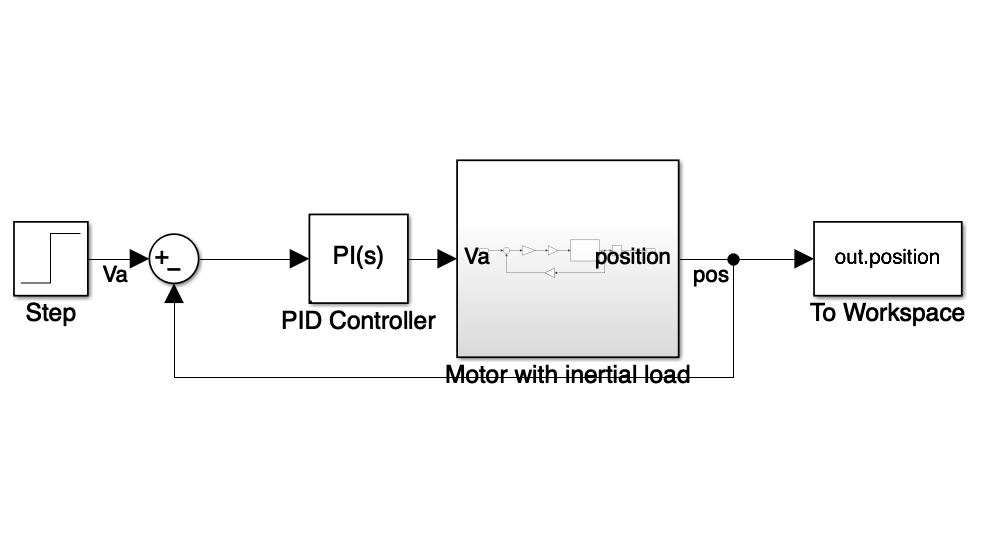
\includegraphics[width=\maxwidth{60.210737581535376em}]{image_6}
\end{flushleft}
\end{par}

\begin{matlabcode}
open_system('TFLoopPI')                     % Load the PI controlled TF model
open_system('motorLoopPI')                  % Load the PI controlled motor model
tfOut = sim('TFLoopPI');
motorOut = sim('motorLoopPI');
figure                                      % Create the position figure
plot(tfOut.position)
hold on
plot(motorOut.position)
hold off
title('TF Vs Motor - PI')
ylabel('Amplitude (rad)')
\end{matlabcode}
\begin{center}
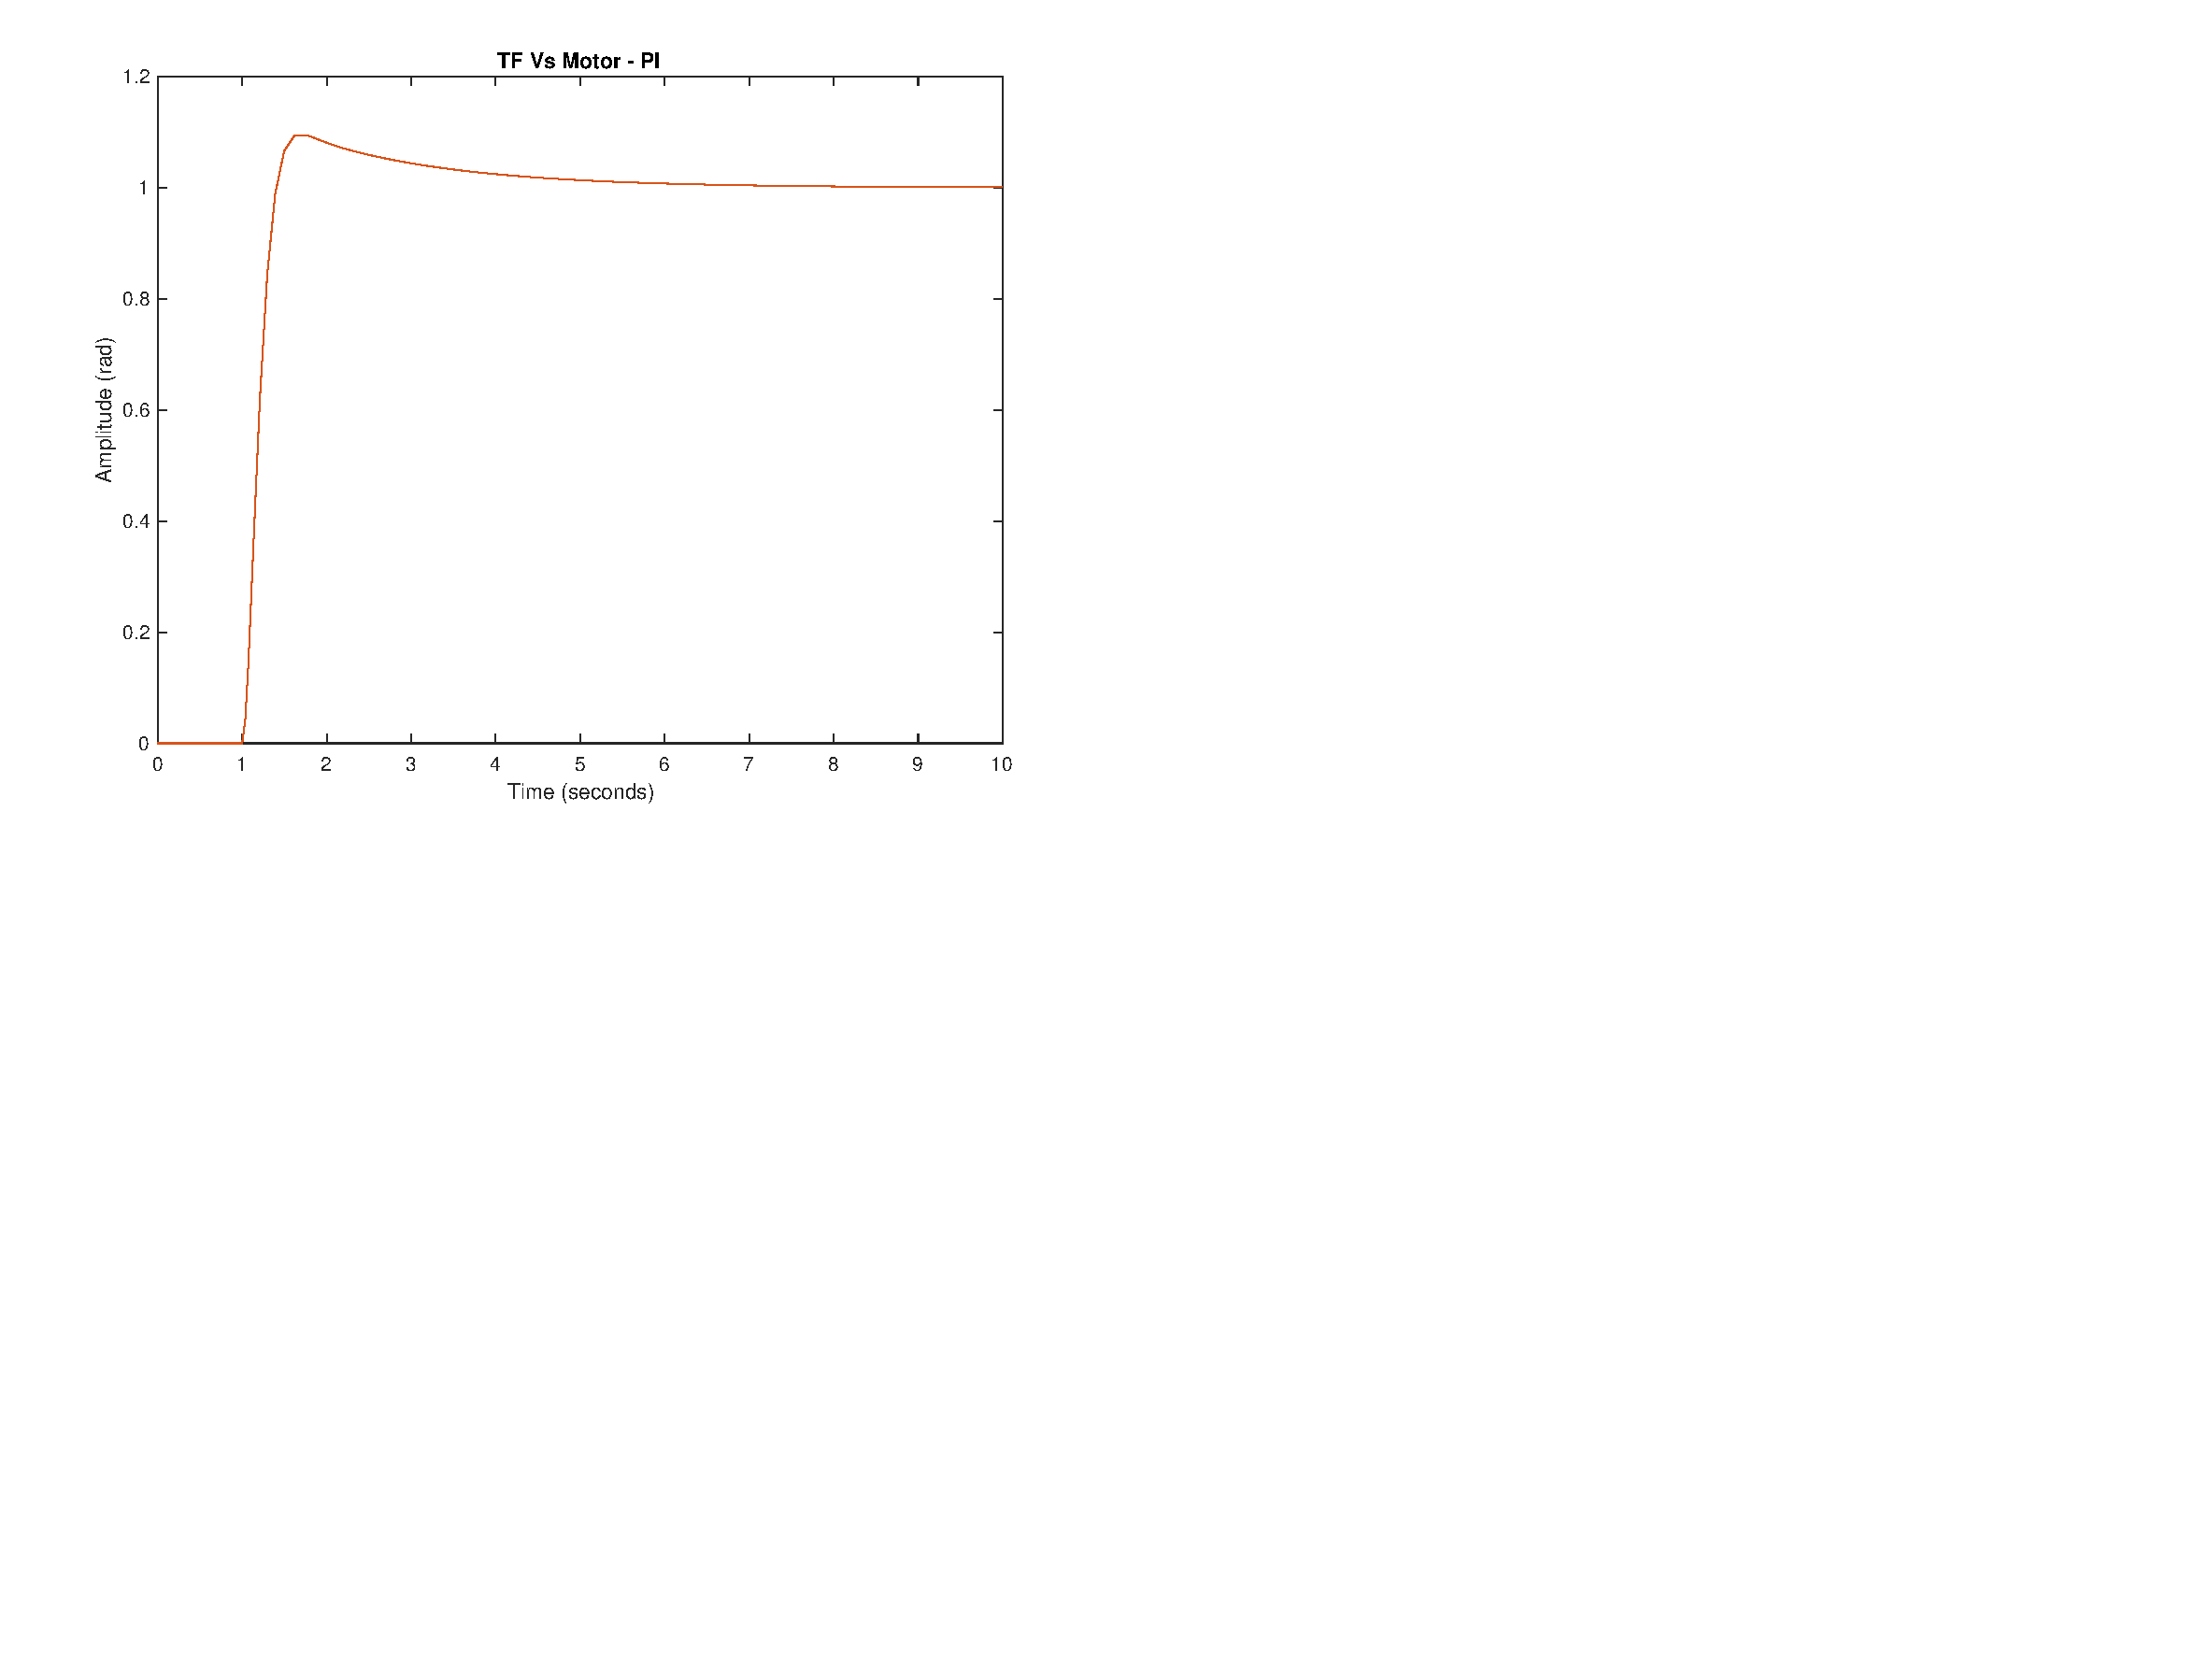
\includegraphics[width=\maxwidth{56.196688409433015em}]{figure_8.eps}
\end{center}


\matlabheadingthree{Tuning a PD Controller for Motor}

\begin{matlabcode}
% Convert Response Time to Bandwidth
% Bandwidth is equivalent to 2 divided by the Response Time
wc2 = 2/0.317841;

% Convert Transient Behavior to Phase Margin
% Phase Margin is equivalent to the Transient Behavior multiplied by 100
PM2 = 100*0.855655;

% Define options for pidtune command
opts2 = pidtuneOptions('PhaseMargin',PM2);

% PID tuning algorithm for linear plant model
[CD,pidInfo2] = pidtune(posTF,'PD',wc2,opts2);

% Clear Temporary Variables
clear wc2 PM2 opts2

% Get desired loop response
Response2 = getPIDLoopResponse(CD,posTF,'closed-loop');

% Plot the result
stepplot(Response2)
title('Step Plot: Reference tracking')
grid on
\end{matlabcode}
\begin{center}
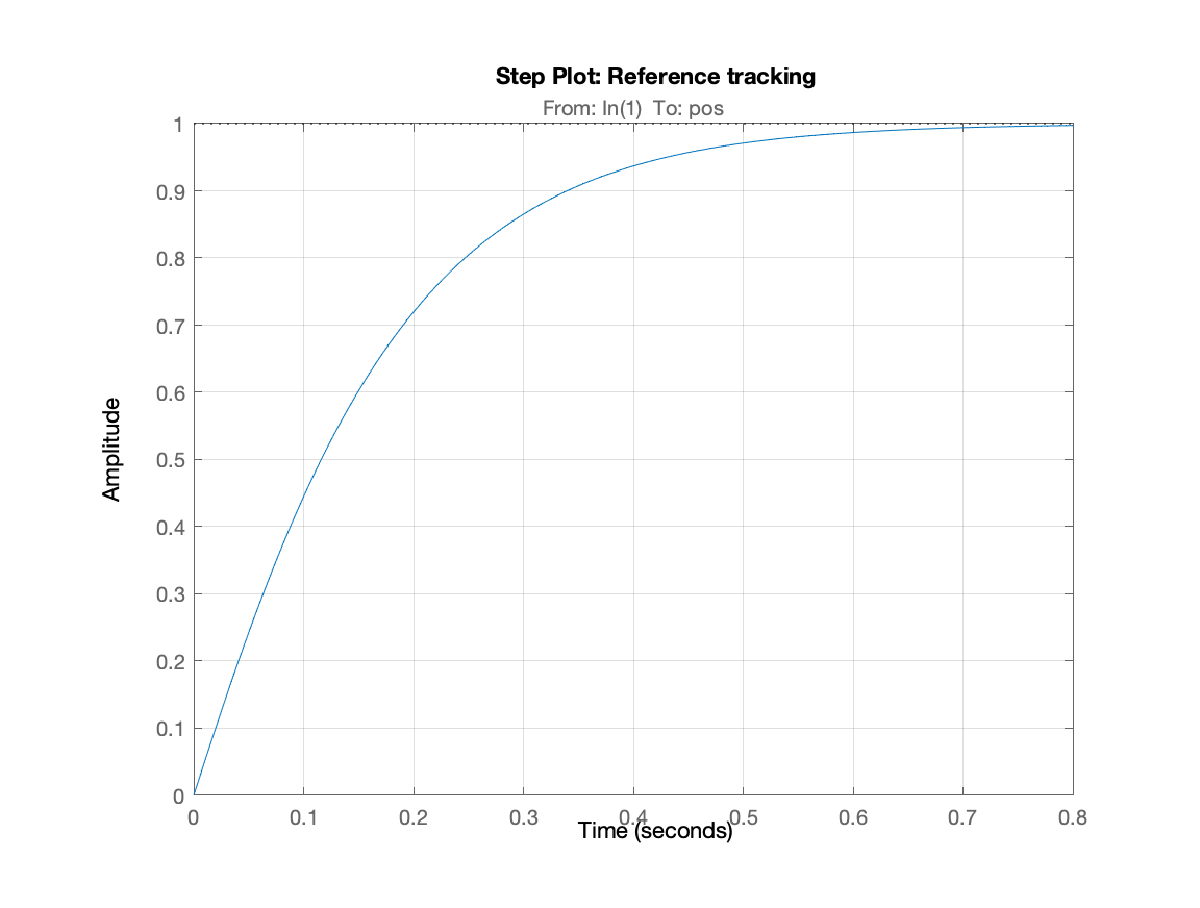
\includegraphics[width=\maxwidth{56.196688409433015em}]{figure_9.eps}
\end{center}
\begin{matlabcode}

% Display system response characteristics
disp(stepinfo(Response2))
\end{matlabcode}
\begin{matlaboutput}
         RiseTime: 0.3200
    TransientTime: 0.5478
     SettlingTime: 0.5478
      SettlingMin: 0.9021
      SettlingMax: 0.9993
        Overshoot: 0
       Undershoot: 0
             Peak: 0.9993
         PeakTime: 0.9652
\end{matlaboutput}
\begin{matlabcode}

% Clear Temporary Variables
clear Response2
Kp = CD.Kp          % Displays the proportial coeficcient
\end{matlabcode}
\begin{matlaboutput}
Kp = 9.7166
\end{matlaboutput}
\begin{matlabcode}
Kd = CD.Kd          % Displays the derivative coeficcient
\end{matlabcode}
\begin{matlaboutput}
Kd = 0.5114
\end{matlaboutput}


\matlabheadingthree{Plot of PD Controlled Motor Vs. Transfer Function - Position}

\begin{par}
\begin{flushleft}
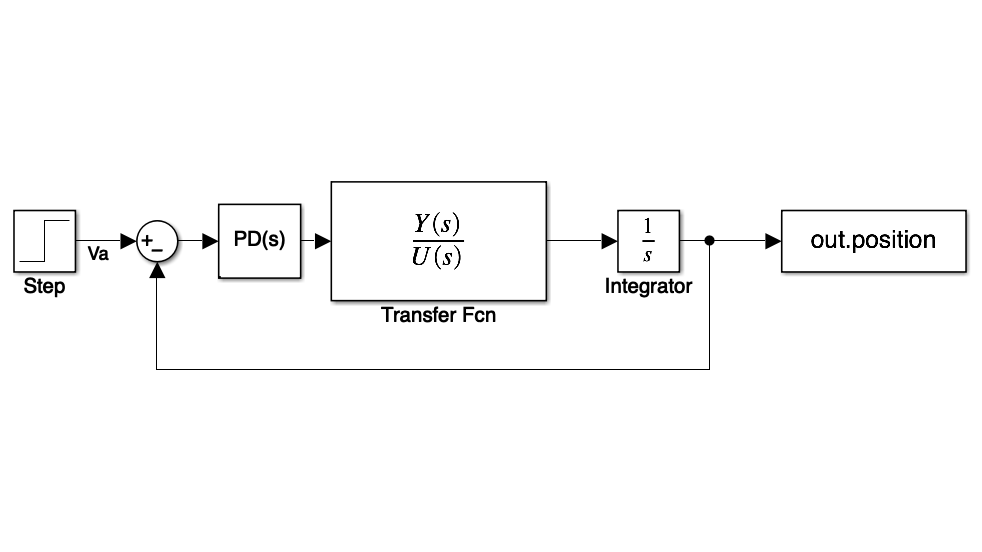
\includegraphics[width=\maxwidth{60.110386352232815em}]{image_7}
\end{flushleft}
\end{par}

\begin{par}
\begin{flushleft}
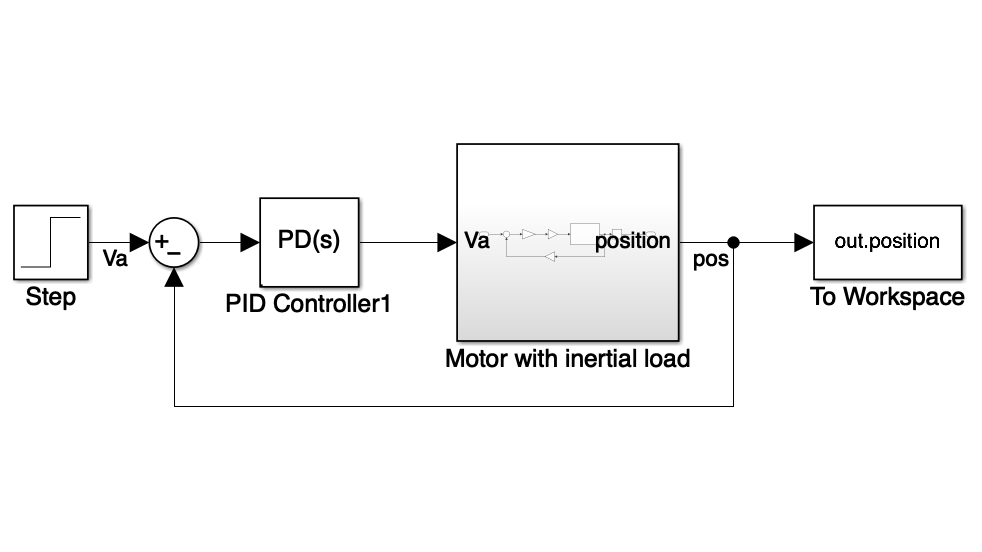
\includegraphics[width=\maxwidth{60.51179126944305em}]{image_8}
\end{flushleft}
\end{par}

\begin{matlabcode}
open_system('TFLoopPD')
open_system('motorLoopPD')
tfOut = sim('TFLoopPD');
motorOut = sim('motorLoopPD');
figure
plot(tfOut.position)
hold on
plot(motorOut.position)
hold off
title('TF Vs Motor - PD')
\end{matlabcode}
\begin{center}
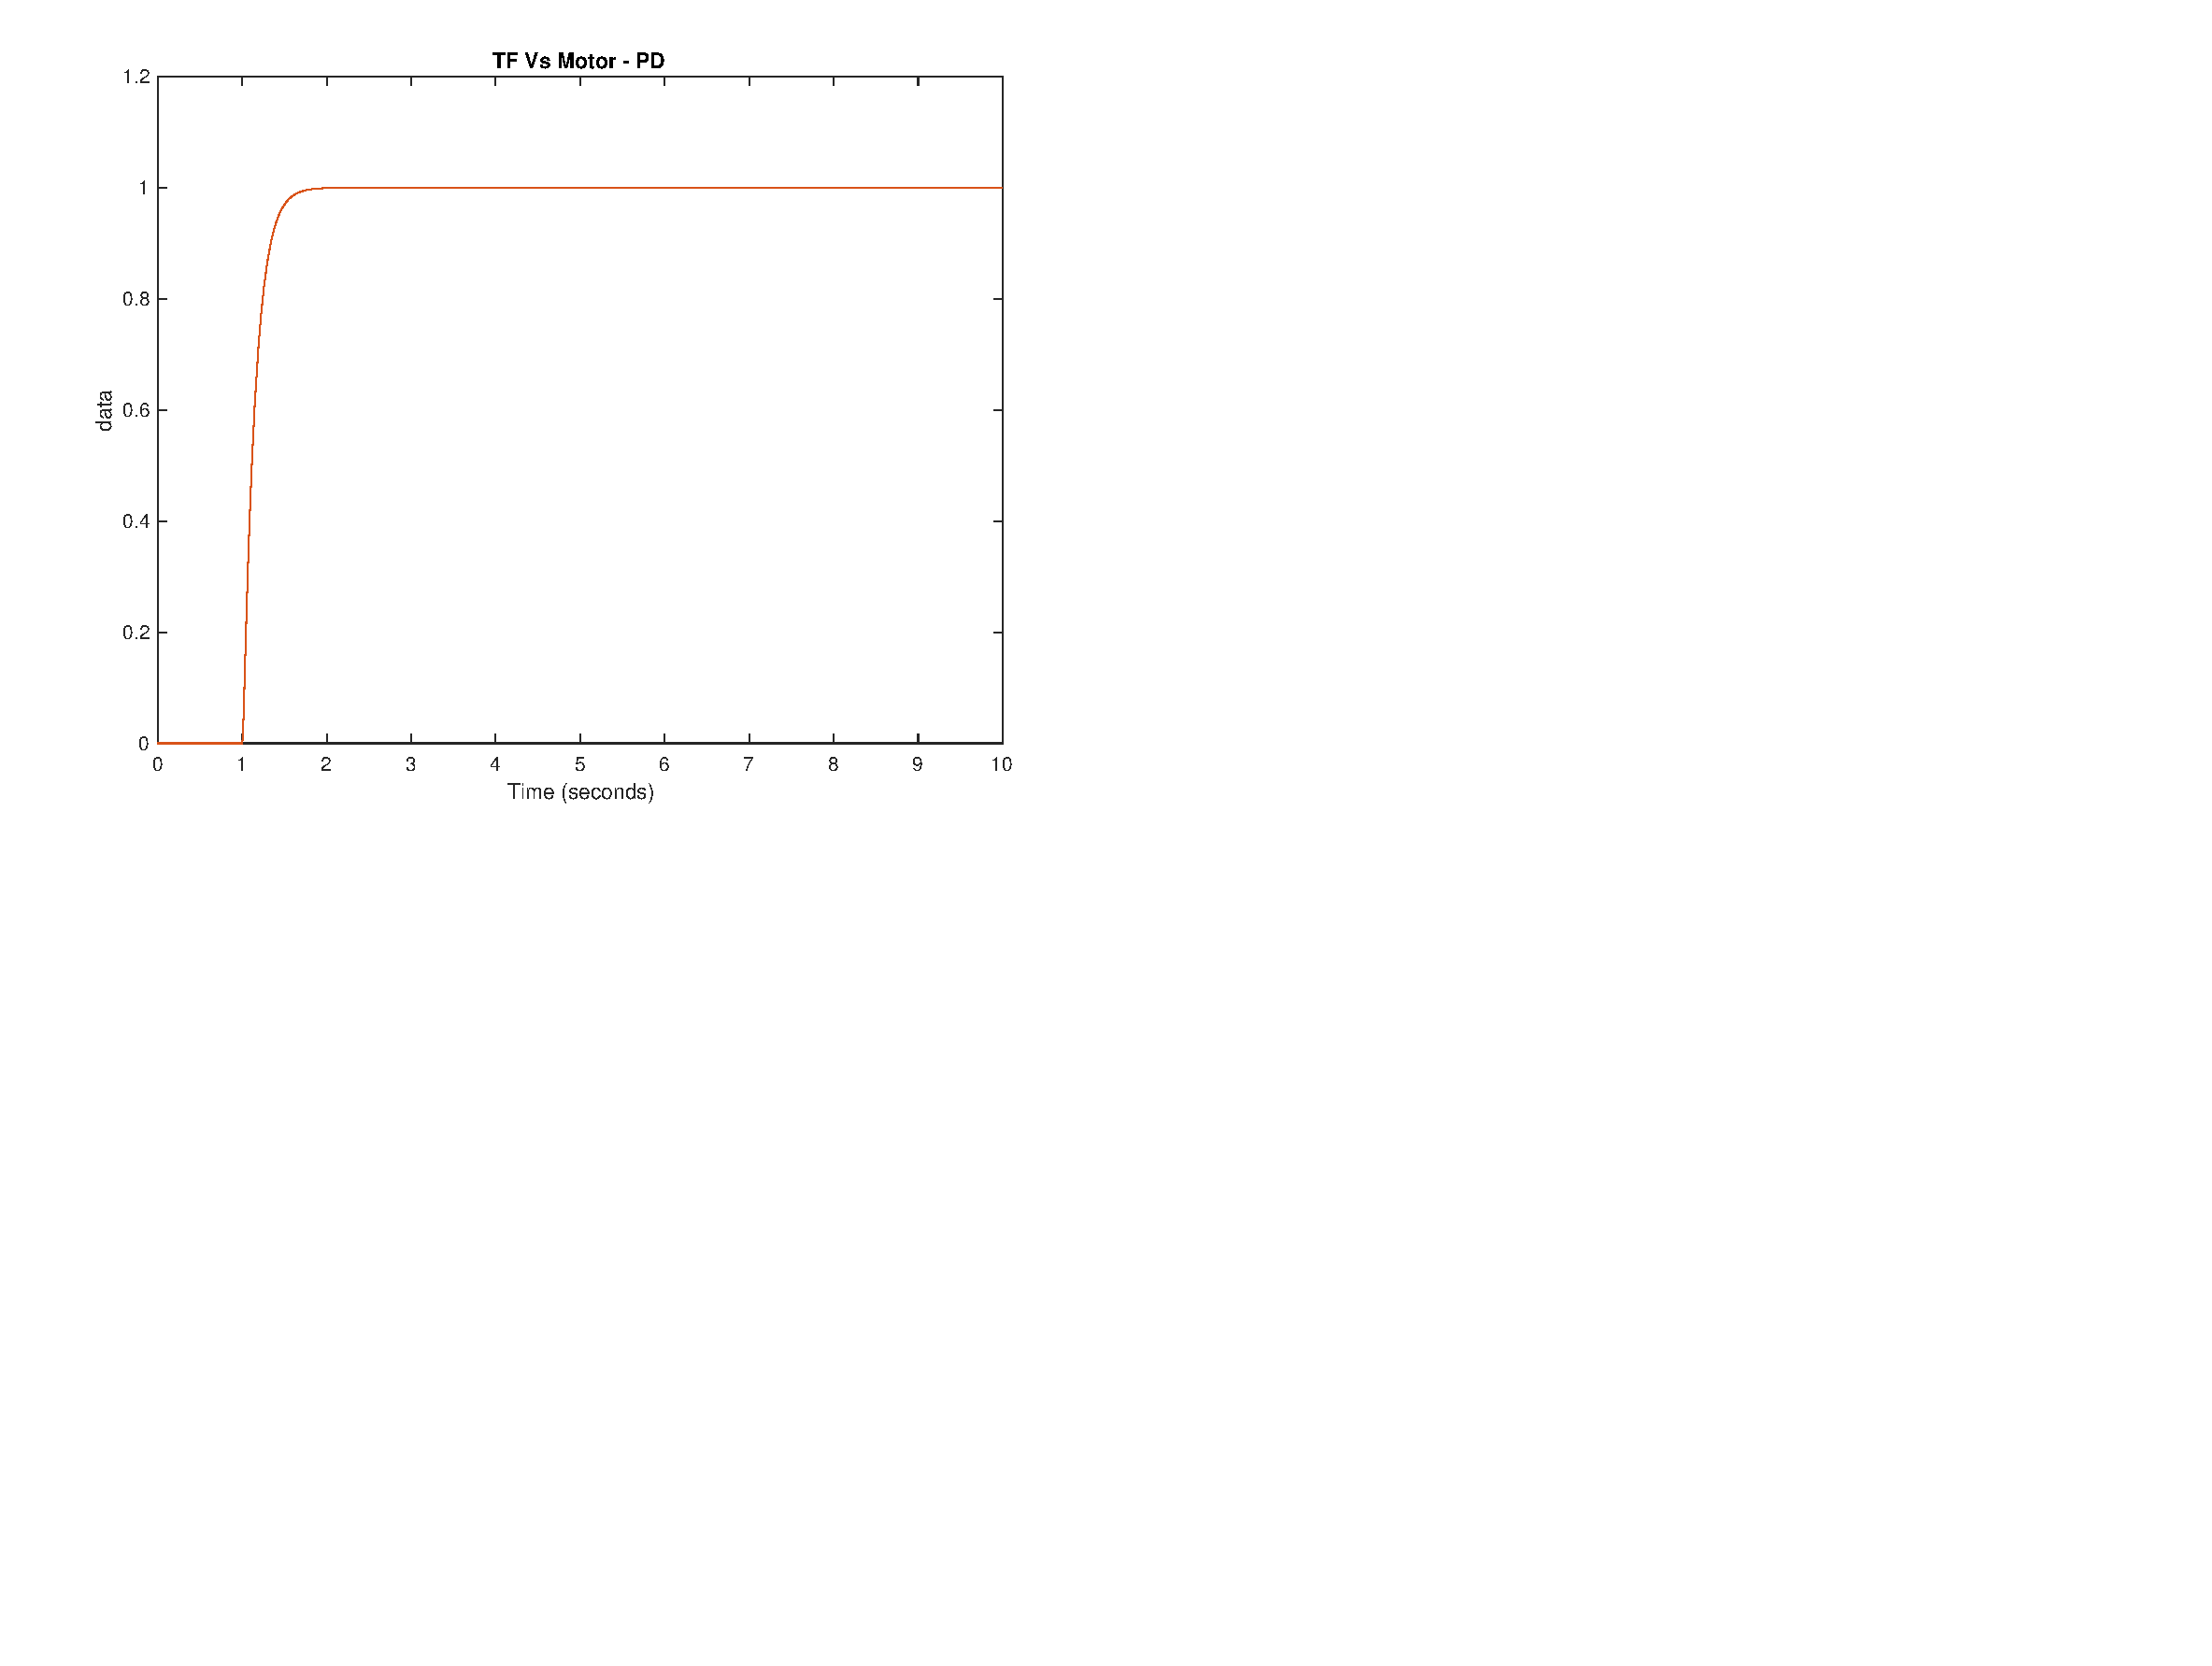
\includegraphics[width=\maxwidth{56.196688409433015em}]{figure_10.eps}
\end{center}

\end{document}
